\documentclass[11pt]{report}
\usepackage[
top    = 2.50cm,% presumably you don't want it to be 0pt as well?
bottom = 2.50cm,
left   = 2cm,
right  = 2cm,
marginparsep = 0pt,
marginparwidth=0pt,
]{geometry}
\usepackage[T1]{fontenc}       % Postscript encoding


\usepackage{lmodern}           % Latin modern for main font

\usepackage{tgadventor}            % Helvetica for headings

\usepackage[scaled=1.03]{inconsolata}   % For ttfamily
%\usepackage{textcomp}
\usepackage{multirow}
\usepackage{standalone}		
\usepackage{fancyhdr}		 %For enabling modular tex file splitting
%\usepackage{indentfirst}			 %Uniform paragraph indentation
\usepackage{pgfplots}                %Tikz and GeoGebra integration
\usepackage{mathrsfs}
%\usepackage{draftwatermark}         %For diagonal watermark
% \usepgfplotslibrary{fillbetween}
\usetikzlibrary{patterns}
\usepackage{commath}
\usepackage{graphicx}
\graphicspath{{pictures/}}
\usepackage{multicol}
\usepackage[most]{tcolorbox}
\usepackage{varwidth}   %% provides varwidth environmen
\usepackage{amsmath,empheq}


\tcbuselibrary{skins}
\usepackage{cancel} %For neat Series Canceling Method
\usepackage{wrapfig}
\usepackage{gensymb}
\makeatletter
\let\savedchap\@makechapterhead
\def\@makechapterhead{\vspace*{-3cm}\savedchap}
\usepackage{amssymb}
\usepackage{setspace}
\usepackage[norndcorners,customcolors]{hf-tikz}
\tikzset{set border color=black,set fill color=white}
\newcommand*{\qe}{$x=\frac{-b\pm\sqrt{b^2-4ac}}{2a}$}
\usepackage[linewidth=1pt]{mdframed}
\usepackage{array}
\usepackage[utf8]{inputenc}
\usepackage{chngcntr}
\usepackage[english]{babel}
%To shift equation tags left and right
\makeatletter
\newcommand{\leqnomode}{\tagsleft@true\let\veqno\@@leqno}
\newcommand{\reqnomode}{\tagsleft@false\let\veqno\@@eqno}
\makeatother
\usepackage{amsmath}

\tikzset{
	mycross/.pic={
		\draw[pic actions] 
		(-3pt,0) -- (3pt,0)
		(0,-3pt) -- (0,3pt);
	},
}


\usepackage{amsthm}
\usepackage[nobottomtitles*]{titlesec}  % For section titles

% Header Setup
\pagestyle{fancy}

\renewcommand{\sectionmark}[1]{\markright{\S\thesection~$|$~#1}}
\renewcommand{\subsectionmark}[1]{\markright{\S\thesubsection~$|$~#1}}
\lhead{\nouppercase\rightmark}
\rhead{\nouppercase\leftmark}
\usepackage{soulutf8} 

\renewcommand{\chaptermark}[1]{%
\markboth{#1}{}}

\cfoot{\thepage}
\rfoot{\footnotesize\scshape Work in Progress}	
	
	\newtcolorbox{mybox}[1][]{before=\centering, drop fuzzy shadow, enhanced, colback=white, sharp corners, colframe=red, fonttitle=\bfseries, title=#1, center title}
	\setlength{\columnseprule}{1pt}
	
	% Title Formats
	\definecolor{gray75}{gray}{0.75}
	\newcommand{\hsp}{\hspace{20pt}}
	\titleformat{\chapter}[hang]{\Huge\bfseries\sffamily}{\thechapter\hsp\textcolor{gray75}{|}\hsp}{0pt}{\Huge\bfseries}
	\titleformat{\section}[hang]{\normalfont\sffamily\LARGE\bfseries}{}{0em}{}
	\titleformat{\subsection}[hang]{\normalfont\sffamily\large\bfseries}{}{0em}{}
	\titleformat{\subsubsection}[hang]{\normalfont\sffamily\bfseries}{}{1em}{}

	% Title spacings
	\titlespacing*{\chapter} {0pt}{1ex plus 1ex minus .2ex}{30pt}
	\titlespacing*{\section} {0pt}{3.5ex plus 1ex minus .2ex}{25pt}
	\titlespacing*{\subsection} {0pt}{3.25ex plus 1ex minus .2ex}{5pt}
	\titlespacing*{\subsubsection} {0pt}{2ex plus 1ex minus .2ex}{2pt}
	
%Adding derivative fraction
\renewcommand\od[2]{\frac{d#1}{d#2}}

\theoremstyle{definition}
\newtheorem{example}{Ex.}
\counterwithin*{example}{section}
\counterwithin*{example}{subsection}


% Allow display breaks
\allowdisplaybreaks
% To avoid `\headhight is too small' warning
\setlength{\headheight}{15pt}

% Swap the definition of \abs* and \norm*, so that \abs
% and \norm resizes the size of the brackets, and the 
% starred version does not.
\makeatletter
\let\oldabs\abs
\def\abs{\@ifstar{\oldabs}{\oldabs*}}
%
\let\oldnorm\norm
\def\norm{\@ifstar{\oldnorm}{\oldnorm*}}
\makeatother

\usepackage{ps-trees}

\setlength{\jot}{13pt}
\usepackage{xstring}	

\setlength\parindent{0em}
\begin{document}
		\documentclass{standalone}
\begin{document}
\begin{titlepage} % Suppresses headers and footers on the title page
		
		\centering % Centre everything on the title page
		
		\scshape % Use small caps for all text on the title page
		
		\vspace*{\baselineskip} % White space at the top of the page
		
		%------------------------------------------------
		%	Title
		%------------------------------------------------
		
		\rule{\textwidth}{1.6pt}\vspace*{-\baselineskip}\vspace*{2pt} % Thick horizontal rule
		\rule{\textwidth}{0.4pt} % Thin horizontal rule
		
		\vspace{0.75\baselineskip} % Whitespace above the title
		
		{\LARGE Pure Mathematics\\Advanced Level} % Title
		
		\vspace{0.75\baselineskip} % Whitespace below the title
		
		\rule{\textwidth}{0.4pt}\vspace*{-\baselineskip}\vspace{3.2pt} % Thin horizontal rule
		\rule{\textwidth}{1.6pt} % Thick horizontal rule
		
		\vspace{2\baselineskip} % Whitespace after the title block
		
		%------------------------------------------------
		%	Subtitle
		%------------------------------------------------
		
		“Once your soul has been enlarged by a truth, it can never return to its original size.”\\
		-Blaise Pascal% Subtitle or further description
		
		\vspace*{3\baselineskip} % Whitespace under the subtitle
		
		%------------------------------------------------
		%	Editor(s)
		%------------------------------------------------
		
		Notes By
		
		\vspace{0.5\baselineskip} % Whitespace before the editors
		
		{\scshape\Large Giorgio Grigolo \\ } % Editor list
		
		\vspace{0.5\baselineskip} % Whitespace below the editor list
		
		\textit{Student of Mathematics and Computer Science \\St.Aloysius College } % Editor affiliation
		
		\vfill % Whitespace between editor names and publisher logo
		
		%------------------------------------------------
		%	Publisher
		%------------------------------------------------
		
		
		\vspace{0.3\baselineskip} % Whitespace under the publisher logo
		
		2020 % Publication year
		
	\end{titlepage}
	\end{document}
		
		\tableofcontents
		\newpage
	
	
	%	\SetWatermarkText{Giorgio G.}
	%	\SetWatermarkScale{5}
	
		%\documentclass{standalone}
\begin{document}
	\chapter{Classification of numbers}
	
	\begin{itemize}
		\item{Natural numbers: $\mathbb{N}$; (1, 2, 3, 4 \ldots)}
		\subitem{This set includes every number which is both positive and whole.}
		\item{Integer numbers: $\mathbb{Z}$; (-2, -1, 0, 1, 2, \ldots)}
		\subitem{The integer number set includes every negative and positive whole numbers, similarly to $\mathbb{N}$}
		\item{Rational numbers: $\mathbb{Q}$; (-1, 2 , $\frac{1}{2}$)}
		\subitem{A number is s.t.b rational if expressed in the form $\frac{p}{q};p, q \in \mathbb{Z}$.}
		\item{Irrational numbers: $\mathbb{Q'}$; ($\pi, e, \sqrt{2}, \sqrt{5}, \ldots$))}
		\subitem{If a number is not classified as any of the above, it is referred to as irrational.}
		\item{Real numbers: $\mathbb{R}$}
		\subitem{Anything mentioned above inclusively represent the set of Real numbers}\\
	\end{itemize}
	
	
	\emph{We can additionally refer to positive or negative numbers in any set by using the notation:}\\
	\begin{center}
		$\mathbb{R}^+$ and $\mathbb{R}^-$
	\end{center}
	%TODO: insert image of sets
	
	
	\newpage	
	\end{document}
		%\documentclass{standalone}
\begin{document}
	\chapter{Surds}
	\section{Introduction}
	\quad Consider numbers $\sqrt{64}, \sqrt{16}$. These can be represented as exact quantities by writing $8$ and $4$. There are however other numbers which cannot be expressed as exact quantities using other symbols.\\
	
	
	There is an option of expressing them as corrected decimals without however preserving their full value. Instead, we choose to keep the form $\sqrt{a}$ which preserves the full value of the numbers.
	\section{Examples}
	\begin{multicols}{2}
		\noindent
		\begin{alignat*}{2}
			a)\quad
			\sqrt{2} & = \sqrt{16\times3}          \\
			& = \sqrt{16} \times \sqrt{3} \\
			& = 4\sqrt{3}                 
		\end{alignat*}
		\begin{alignat*}{2}
			b)\quad
			\sqrt{72} & = \sqrt{8\times9}         \\
			& = \sqrt{9}\times \sqrt{8} \\
			& = 3\sqrt{8}               
		\end{alignat*}
		\begin{alignat*}{2}
			\quad
			\sqrt{360} & = \sqrt{180} \times \sqrt{2} \\
			& =\sqrt{36}\times\sqrt{10}    \\
			& =6\sqrt{10}                  
		\end{alignat*}
		\begin{alignat*}{2}
			d)\quad
			& \quad\left(1+2\sqrt{3}\right)\left(2+3\sqrt{5}\right) \\
			& = 2-\sqrt{3}  - 10\sqrt{3}                            \\
			& =-28-\sqrt{3}                                         
		\end{alignat*}
		\begin{alignat*}{2}
			e)\footnote[1]\quad
			& \quad\left(2-3\sqrt{5}\right)\left(2+3\sqrt{5}\right) \\
			& = 4+6\sqrt{5}-6\sqrt{5}-9(5)                          \\
			& =-41                                                  
		\end{alignat*}
	\end{multicols}
	\footnotetext[1]{This expression shows that for products of the form $\left(a+b\sqrt{c}\right)\left(a-b\sqrt{c}\right)$ the surds will vanish.}
	\newpage
	\section{Rationalizing the denominator}
	\quad \emph{Consider the fraction:} 
	$$\frac{1}{1+\sqrt{2}}$$
	This fraction contains a surd, thus, making it irrational. To rationalize said fraction one should find the multiplicative operation of canceling the denominator \textit{(see \footnotemark[1])}.\\
	
	
	\emph{Continuing...}
	\begin{alignat*}{2}
		\frac{1}{1+\sqrt{2}} & = \frac{1}{1+\sqrt{2}} \times \frac{1-\sqrt{2}}{1-\sqrt{2}} \\
		& =\frac{1-\sqrt{2}}{1}                                       \\
		& =1-\sqrt{2}                                                 
	\end{alignat*} 
\end{document}
		%	\documentclass{standalone}
	\begin{document}
	\chapter{Partial Fractions}
	\section{Introduction}
	\emph{Consider the expression and suppose it is simplified:}
	
	
	\begin{alignat*}{2}
		\frac{2}{x+1}+\frac{3}{2x-5} & = \frac{2(2x-5)+3(x+1)}{(x+1)(2x-5)} \\
		& =\frac{4x-10+3x+3}{(x+1)(2x-5)}      \\
		& =\frac{4x-10+3x+3}{(x+1)(2x-5)}      \\
		& =\frac{7x-7}{(x+1)(2x-5)}            \\
	\end{alignat*}
	
	In this chapter we reverse the approach above, hence decomposing one fraction to its corresponding partial fractions.
	\newpage
	\section{Types of partial fraction cases}
	\subsection*{\underline{Type 1: Linear Factors in denominator}}
	\begin{example}
		Decompose $ \frac{7x-7}{\left(x+1\right)}$ into Partial Fractions
	\end{example}
	\begin{alignat*}{2}	
		&            & \frac{7x-7}{\left(x+1\right)} & \equiv \frac{A}{\left(x+1\right)} + \frac{B}{\left(2x-5\right)} \\
		& \implies   & 7x-7                          & = A\left(2x-5\right)+B\left(x+1\right))                         \\	
		& \implies   & 7(-1)-7                       & = A(2(-1)-5)\tag*{$x = -1$}                                     \\
		& \implies   & -14                           & = -7A                                                           \\\leqnomode
		& \implies   & A                             & = 2\tag{..1}                                                    \\
		& \implies   & 7\left(\frac{5}{2}\right)-7   & =B\left(\left(\frac{5}{2}\right)+1\right)\tag*{$x=\frac{5}{2}$} \\
		& \implies   & \frac{35}{2} - 7              & = \frac{7B}{2}                                                  \\
		& \implies   & B                             & =3\tag{..2}                                                     \\\\
		& \therefore & \frac{7x-7}{\left(x+1\right)} & = \frac{2}{\left(x+1\right)} + \frac{3}{\left(2x-5\right)}      
	\end{alignat*}
	
	
	\subsection*{\underline{Type 2: Irreducible Quadratic Factor in Denominator}}
	\begin{example}
		Decompose $\frac{x^2 +1}{(2x+1)(x^2 +3)}$ into its corresponding partial fractions.
	\end{example}
	\begin{alignat*}{2}
		&            & \frac{x^2 +1}{(2x+1)(x^2 +3)} & \equiv \frac{A}{2x+1}+\frac{Bx+C}{x^2 +3}       \\
		& \implies   & x^2 + 1                       & \equiv A(x^ 2 + 3) + (Bx+C)(2x+1)               \\
		& \implies   & x^2 + 1                       & \equiv x^2(A+2B) + x(2B + 2C) + (3A+C)\tag{*..} \\
		\intertext{\quad At this stage, since both equations are identical, we analyse the different coefficients and constants to form a system of equations to solve.}
		\intertext{Comparing coefficients of $x^2\colon$}
		&            & 1                             & = A+2B\tag{1..}                                 \\
		\intertext{Comparing coefficients of $x\colon$}
		&            & 0                             & = B+C\tag{2..}                                  \\
		\intertext{Comparing constants$\colon$}
		&            & C                             & = 1-3A\tag{3..}                                 \\
		\intertext{Substituting  3.. in 2..}
		&            & 0                             & =B+1-3A                                         \\
		& \implies   & B                             & =3A-1\tag{4..}                                  \\
		\intertext{Substituting 4.. in 1..}
		&            & 1                             & = A + 2(3A-1)                                   \\
		& \implies   & A                             & = \frac{-1}{7} \tag{5..}                        \\
		\intertext{Substituting 5.. in 1..}
		&            & 1                             & = \frac{-1}{7} +2B                              \\
		& \implies   & -7                            & = 1-14B                                         \\
		& \implies   & B                             & =\frac{4}{7}\tag{6..}                           \\
		\intertext{Substituting 5.. in 3..}
		&            & C                             & = 1-3\left(\frac{-1}{7}\right)                  \\
		& \implies   & C                             & = \frac{10}{7}                                  \\
		& \therefore & \frac{x^2 +1}{(2x+1)(x^2 +3)} & \equiv \frac{A}{2x+1}+\frac{Bx+C}{x^2 +3}       
	\end{alignat*}
	\newpage
	\subsection*{\underline{Type 3: Repeated factor in the denominator}}
	\begin{example}
		Decompose $\frac{x+1}{(x+2)(x-3)^2}$ into its corresponding partial fractions.
	\end{example}
	\begin{alignat*}{2}
		&            & \frac{x+1}{(x+2)(x-3)^2} & \equiv \frac{A}{x+2} + \frac{B}{x-3} + \frac{C}{(x-3)^2}           \\
		& \implies   & x+1                      & \equiv A(x-3)^2 + B(x-3)(x+2) + C(x+2)                             \\
		& \implies   & x+1                      & \equiv Ax^2 - 6Ax +9A + Bx^2-Bx-6B + Cx+2C)                        \\
		& \implies   & -2+1                     & =A(-2-3)^2\tag*{$x=-2$}                                            \\
		& \implies   & A                        & = \frac{-1}{25}                                                    \\
		& \implies   & 3+1                      & =C(3+2)\tag*{$x=3$}                                                \\
		& \implies   & C                        & =\frac{4}{5}                                                       \\
		\intertext{Comparing coefficients of $x^2\colon$}
		& \implies   & 0                        & = A + B                                                            \\
		& \implies   & B                        & = \frac{1}{25}                                                     \\
		& \therefore & \frac{x+1}{(x+2)(x-3)^2} & \equiv \frac{1}{25(x-3)} + \frac{4}{5(x-3)^2} - \frac{-1}{25(x-3)} \\
	\end{alignat*}
	
	The approach above, is similar to the previous one, with the addition of the fact that each repeated factor has to be listed in order of powers until its own.
	\newpage
	\subsection*{\underline{Type 4: Improper fraction}}
	\begin{example}
		Decompose $\frac{2x^2 -8x +11}{2x-5}$ into its corresponding partial fractions.
	\end{example}
	Since the fraction is improper, or top-heavy\footnotemark[2] it is required to perform a polynomial long division and acquire the proper terms. \footnotetext[2]{Improper fractions containing a variable are recognized by the order of the exponent when the expression is expanded. i.e $\frac{x^2}{x+5}$ is regarded as improper}
	\begin{center}
		\polylongdiv{2x^2 -8x +11}{2x-5}
	\end{center}
	\begin{alignat*}{2}
		& \therefore\quad & \frac{2x^2 -8x +11}{2x-5} & \equiv 	x - \frac{3}{2} + \frac{7}{2(2x-5)} 
	\end{alignat*}
	\newpage
	\end{document}
		%\documentclass{standalone}
\begin{document}
	\chapter{Pascal's Triangle}
	\bigskip
	\emph{Consider the following expansions:}
	\begin{gather*}
		(1+x)^0 = 1\\
		(1+x)^1 = 1+x\\
		(1+x)^2 = 1+2x+x^2\\
		(1+x)^3 = 1+3x+3x^2+x^3\\
		(1+x)^4 = 1+4x+6x^2+4x^3+x^4\\
		(1+x)^5 = 1+5x+10x^2+10x^3+5x^4+x^5\\
		(1+x)^6 = 1+6x+15x^2+20x^3+15x^4+6x^5+x^6\\
		\ldots\\
		\begin{tabular}{>{$n=}l<{$\hspace{12pt}}*{13}{c}}
			&   &   &   &   &    &    & 1  &    &    &   &   &   &   \\
			&   &   &   &   &    & 1  &    & 1  &    &   &   &   &   \\
			&   &   &   &   & 1  &    & 2  &    & 1  &   &   &   &   \\
			&   &   &   & 1 &    & 3  &    & 3  &    & 1 &   &   &   \\
			&   &   & 1 &   & 4  &    & 6  &    & 4  &   & 1 &   &   \\
			&   & 1 &   & 5 &    & 10 &    & 10 &    & 5 &   & 1 &   \\
			6 & 1 &   & 6 &   & 15 &    & 20 &    & 15 &   & 6 &   & 1 
		\end{tabular}
	\end{gather*}\\
	The above array of numbers is called Pascal's Triangle. It can be used to expand any binomial. The following examples illustrate its use.\\
	\newpage
	\begin{example}
		Expand the following using Pascal's Triangle
	\end{example}
	\begin{alignat*}{2}
		(1+2x)^5                      & \equiv 1(2x)^0 + 5(2x)^1 + 10(2x)^2 + 10(2x)^3 + 5(2x)^4 + 2x^5\tag*{a)}                                                                          \\
		& \equiv 1 + 10x + 40x^2 + 80x^3 + 80x^4 + 32x^5                                                                                                    \\
		\\	
		\left(1-\frac{3x}{2}\right)^6 & \equiv 1\left(\frac{-3x}{2}\right)^0 + 6\left(\frac{-3x}{2}\right)^1 + 15\left(\frac{-3x}{2}\right)^2 + 20\left(\frac{-3x}{2}\right)^3 +\tag*{b)} \\
		& \quad 15\left(\frac{-3x}{2}\right)^4 + 6\left(\frac{-3x}{2}\right)^5 + 1\left(\frac{-3x}{2}\right)^6                                              \\
		& \equiv 1 - 9x + \frac{135x^2}{4} - \frac{135x^3}{2} + \frac{1215x^4}{16} - \frac{243x^5}{16} + \frac{728x^6}{64}                                  \\
		&   \\(p+q)^4 &\equiv (p(1+\frac{q}{p}))^4\tag*{c)}\\
		& \equiv p^4\left(1+\frac{q}{p}\right)^4                                                                                                            \\
		& \equiv p^4\left(1 + \frac{4q}{p} + \frac{6q^2}{p^2} + \frac{4q^3}{p^3} + \frac{q^4}{p^4}\right)                                                   \\
		& \equiv p^4 + 4p^3q + 6p^2q^2 + 4pq^3 + q^4                                                                                                        
	\end{alignat*}
	In the above examples we observe that: 
	
	\begin{itemize}
		\item{The expansion contains the coefficients for Pascal's Triangle.}
		\item{The expansion is formed by descending exponents of the first term of the binomial \& ascending exponents of the second.}
		\item{The sum of the exponents in each term is equal to the 	exponent by which the binomial was raised.}
	\end{itemize}
	These observations can be applied to expand any binomials raised with positive integer exponents.	
\end{document}
		%\documentclass{standalone}
\begin{document}
	\chapter{The Remainder and Factor Theorems}
	\section{The Remainder Theorem}
	Consider the polynomial $f(x)$. Suppose that this polynomial is to be divided by the linear expression $x-a$. This gives:
	\begin{alignat*}{3}
		&&\frac{f(x)}{x-a}A&\equiv Q(x) + \frac{R}{x-a}\\
		&\implies&f(x) &\equiv Q(x) \cdot (x-a) + R\\
		\text{Let $x-a=0$}&\implies &x &= a\\
		& \therefore & f(a) & = R;\quad & \text{Where R is the remainder of $\frac{f(x)}{x-a}$} \\
		&            &      &           & \text{and Q is the quotient of $\frac{f(x)}{x-a}$}    \\
	\end{alignat*} \\
	\begin{example}
		Find the remainder when the cubic polynomial $f(x) = 2x^3-3x-5$ is divided by $x-2$
	\end{example}
	
	
	If $f(x)$ is to be divided by $x-2$, then $f(2)$ is equal to the remainder of $\frac{2x^3-3x-5}{x-2}$
	\begin{alignat*}{2}
		&        & 2x^3 -3x-5       \\
		& =\quad & 2(2)^3 - 3(2) -5 \\
		&\boxed{\therefore\quad R\quad=\quad5}
	\end{alignat*}
	\section{The Factor theorem}
	
	The factor theorem states that:
	\begin{itemize}
		\item{If the polynomial $f(x)$ is divided by $x-a$, then $f(a) = 0$ (i.e $R=0$}), therefore it can also be concluded that $x-a$ is a factor of $f(x)$
	\end{itemize}
	\begin{example}
		Determine whether $2x+3$ is a factor of $2x^3+x^2-5x+6$ 
	\end{example}
	
	\begin{flalign*}
		&  & \text{Let } f(x) &= 2x^3+x^2-5x+6& \\
		& \rlap{If $2x+3$ is a factor of $f(x)\colon$} &0 &=f\left(\frac{-3}{2}\right)\\
		&\rlap{However,} &0 &\neq 2\left(\frac{-3}{2}\right)^3 + \left(\frac{-3}{2}\right)^2 -5\left(\frac{-3}{2}\right) + 6 \\
		&&&\neq -3\\
		&&&\boxed{\therefore \quad \text{$2x+3$ is \textbf{not} a factor of $f(x)$}}
	\end{flalign*}
	\newpage
	\end{document}
		%\documentclass{standalone}
\begin{document}
	\chapter{Quadratic Equations}
	\section{Definition}
	\quad A quadratic equation is of the form $ax^2+bx+c=0$ where $a,b,c \in \mathbb{R},\quad a\neq0$. These can be solved algebraically using one of the following methods:
	\begin{itemize}		
		\item{Fractions}
		\item{Completing the square}
		\item{The quadratic formula\footnote[3]{\qe}}
	\end{itemize}
	\section{Nature of roots of the Quadratic Equation}
	\quad Any quadratic equation has in general two roots, namely \qe.
	The quantity $b^2-4ac$ determines the nature of these roots.
	\begin{itemize}
		\item{$b^2-4ac > 0\colon$ Equation holds two real and distinct roots.}
		\item{$b^2-4ac = 0\colon$ Equation holds two equal\footnote[4]{It is implied that they are real.} roots.}
		\item{$b^2-4ac > 0\colon$ Equation holds two complex roots.}
	\end{itemize}
	\quad Thus, the quantity $b^2-4ac$ discriminates among the type of roots that a quadratic equation may have. Therefore it is called the discriminant.
	\begin{example}
		Determine, without solving the nature of the following function.
	\end{example}
	\begin{alignat*}{2}
		& Let        & f(x) =                 & 2x^2+3x-17                              \\
		& \implies   & b^2-4ac                & =3^2-4(2)(-17)                          \\
		&            &                        & = 145                                   \\
		&            &                        & > 0                                     \\
		& \therefore & \text{Roots of $f(x)$} & \in \mathbb{R} \text{ and are distinct} 
	\end{alignat*}
	\hrulefill
	\begin{example}
		Determine the value of $p$ if $ px^2-10x+1 = 0 $ has two equal roots
	\end{example}
	
	Given that the equation has two equal roots:
	
	\begin{alignat*}{2}
		&          & b^2-4ac                        & = 0 \\
		& \implies & 100-4p                         & = 0 \\
		&          & \boxed{\therefore \quad p = 5} &     
	\end{alignat*}
	
	\newpage
	\section{Roots and Coefficients of a Quadratic Equation}
	\subsection{Proof}
	\emph{Consider a general quadratic equation:}
	\begin{alignat*}{2}
		&            & ax^2+bx+c                            & = 0 \tag{1..}                              \\
		& \implies   & x^2 +\frac{bx}{a} + \frac{c}{a}      & = 0                                        \\
		\intertext{Let $\alpha$  and $\beta$  be the roots:}
		& \implies   & (x-\alpha)(x-\beta)                  & = 0                                        \\
		& \implies   & x^2 -\beta x -\alpha x + \alpha\beta & = 0                                        \\
		& \implies   & x^2-(\alpha + \beta)x + \alpha\beta  & = 0\tag{2..}                               \\
		\intertext{Since (1..) and (2..) are identical:}
		& \implies   & x^2 +\frac{bx}{a} + \frac{c}{a}      & \equiv x^2-(\alpha + \beta)x + \alpha\beta \\
		& \therefore & \alpha + \beta                       & = \frac{-b}{a}                             \\ 
		&            & \alpha\beta                          & = \frac{c}{a}                              
	\end{alignat*}
	\hrulefill
	
	\begin{example}
		Write down the quadratic equation whose roots have a sum of 7 \& a product of 5.
	\end{example}
	\begin{alignat*}{2}
		&   &        & x^{2} - (\alpha + \beta) + (\alpha\beta) \\
		&   & =\quad & x^2 - 7x + 7                             
	\end{alignat*}
	\hrulefill
	\begin{example}
		The roots of the equation $2x^2 + 5x -1$ are $\alpha$ and $\beta$. Find the equation whose roots are $\frac{1}{\alpha} $ \& $\frac{1}{\beta}$
	\end{example}
	\begin{alignat*}{2}
		&   & \alpha + \beta & = \frac{-5}{2} \\
		&   & \alpha\beta    & = \frac{-1}{2} 
	\end{alignat*}
	\newpage
	\begin{multicols}{2}
		\textit{Sum of roots:}
		\begin{alignat*}{2}
			&   &   & \frac{1}{\alpha} + \frac{1}{\beta} \\
			&   & = & \frac{\alpha+\beta}{\alpha\beta}   \\
			&   & = & \frac{-5}{2} \div \frac{-1}{2}     \\
			&   & = & 5                                  
		\end{alignat*}
		\textit{Product of roots:}
		
		\begin{alignat*}{2}
			\\&&&\frac{1}{\alpha\beta}\\
			&   & = & \frac{-2}{1} \\
			&   & = & -2           
		\end{alignat*}
	\end{multicols}
	\[ 
	\therefore \quad f(x) = x^2-5x-2
	\]
	\newpage
	
	\end{document}
		%\documentclass{standalone}
\begin{document}
		\chapter{Logarithms}
	\section{Definition}
	\quad In mathematics, the logarithm is the inverse function to exponentiation. That means the logarithm of a given number $x$ is the exponent to which another fixed number, the base $b$, must be raised, to produce that number $x$.\\
	
	\emph{Consider: }\\$$ 2^3 = 8$$\\
	
	3 is the exponent by which 2 must be raised to obtain 8. This statement can also be reversed:\\ 3 is the logarithm by which with a base of 2, results in 8. Thus:$$ 3 = \log_28$$\\
	
	\emph{In general: }\\$$a^b = c \iff \log_ac = b ,\quad a \in \mathbb{R^+}$$\\
	
	
	Furthermore, it is standard to represent $\log_{10}(x)$ as $\log(10) $ and $ \log_e(x) $ as $ \ln(x) $
	
	
	\bigskip
	\bigskip
	\bigskip
	\bigskip
	
	\tcbset{
		enhanced,
		colback=red!5!white,
		boxrule=0.1pt,
		colframe=black!75!black,
		fonttitle=\bfseries
	}
	\begin{center}
		\begin{tcolorbox}[center title,hbox,    %%<<---- here
			lifted shadow={1mm}{-2mm}{3mm}{0.1mm}%
			{black!50!white}]
			\begin{varwidth}{\textwidth}
				\begin{center}
					$	\log_a1                         = 0                    $ \\
					\bigskip
					$\log_aa                          = 1                    $ \\
					\bigskip
					$	\log_c(ab)                       \equiv \log_ca + log_cb $\\
					\bigskip
					$	\log_c\left (\frac{a}{b}\right)  \equiv \log_ca - log_cb$ \\
					\bigskip
					$	n\log_ca                         \equiv \log_ca^n   $     
				\end{center}
			\end{varwidth}
		\end{tcolorbox} 
	\end{center}
	\section{Proofs}
	
	
	
	\paragraph{Proof 1: }$\log_aa  = 1$
	\begin{center}
		$	\text{Let} \log_aa = x$
		$$   a^x      = a $$
		$$x        =1 $$
	\end{center}
	\paragraph{Proof 2: }$\log_aa  = 1$
	\begin{center}
		$	\text{Let} \log_a1 = x$
		$$   a^x      = 1 $$
		$$x        = 0$$
	\end{center}
	\paragraph{Proof 3: }$\log_cab  = \log_ca + \log_cb$
	\begin{center}
		$	\text{Let} \log_ca = x$ ; $\text{Let} \log_cb = y$
		$$\Rightarrow  c^{x} = a  \text{ ; } c^{y} = b$$
		$$\Rightarrow ab = c $$
		$$\Rightarrow\log_c(ab) = \log_c(x) + \log_c(y)$$
		$$\therefore\quad \log_c(ab) = \log_c(a) + \log_c(b)$$
	\end{center}
	\paragraph{Proof 4: }$\log_c\frac{a}{b}  = \log_ca - \log_cb$
	\begin{center}
		$	\text{Let} \log_ca = x$ ; $\text{Let} \log_cb = y$
		$$  c^{x} = a  \text{ ; } c^{y} = b$$
		$$\frac{a}{b} = c^x \times c^{-y} $$
		$$\log_c\frac{a}{b} = \log_c(x) - \log_c(y)$$
	\end{center}
	\paragraph{Proof 5: }$\log_ca^n = n\log_ca$
	\begin{center}
		$	\text{Let} \log_ca^n = x$
		$$ c^x = a^n$$
		$$c^{\frac{x}{n}} = a  $$
		$$\log_ca = \frac{x}{n}$$
		$$x = n\log_ca $$
	\end{center}
\end{document}
		%\documentclass{standalone}
\begin{document}
	\chapter{Vectors}
	\section{Definition}
	\quad A vector quantity is one which has magnitude and direction. For example, length is defined only by size and therefore is a \textit{scalar quantity}. However, acceleration due to gravity, while having a known magnitude, it is also acting in a particular direction. Hence, acceleration is a vector quantity.
	
	\begin{wrapfigure}{r}{0.25\textwidth}
		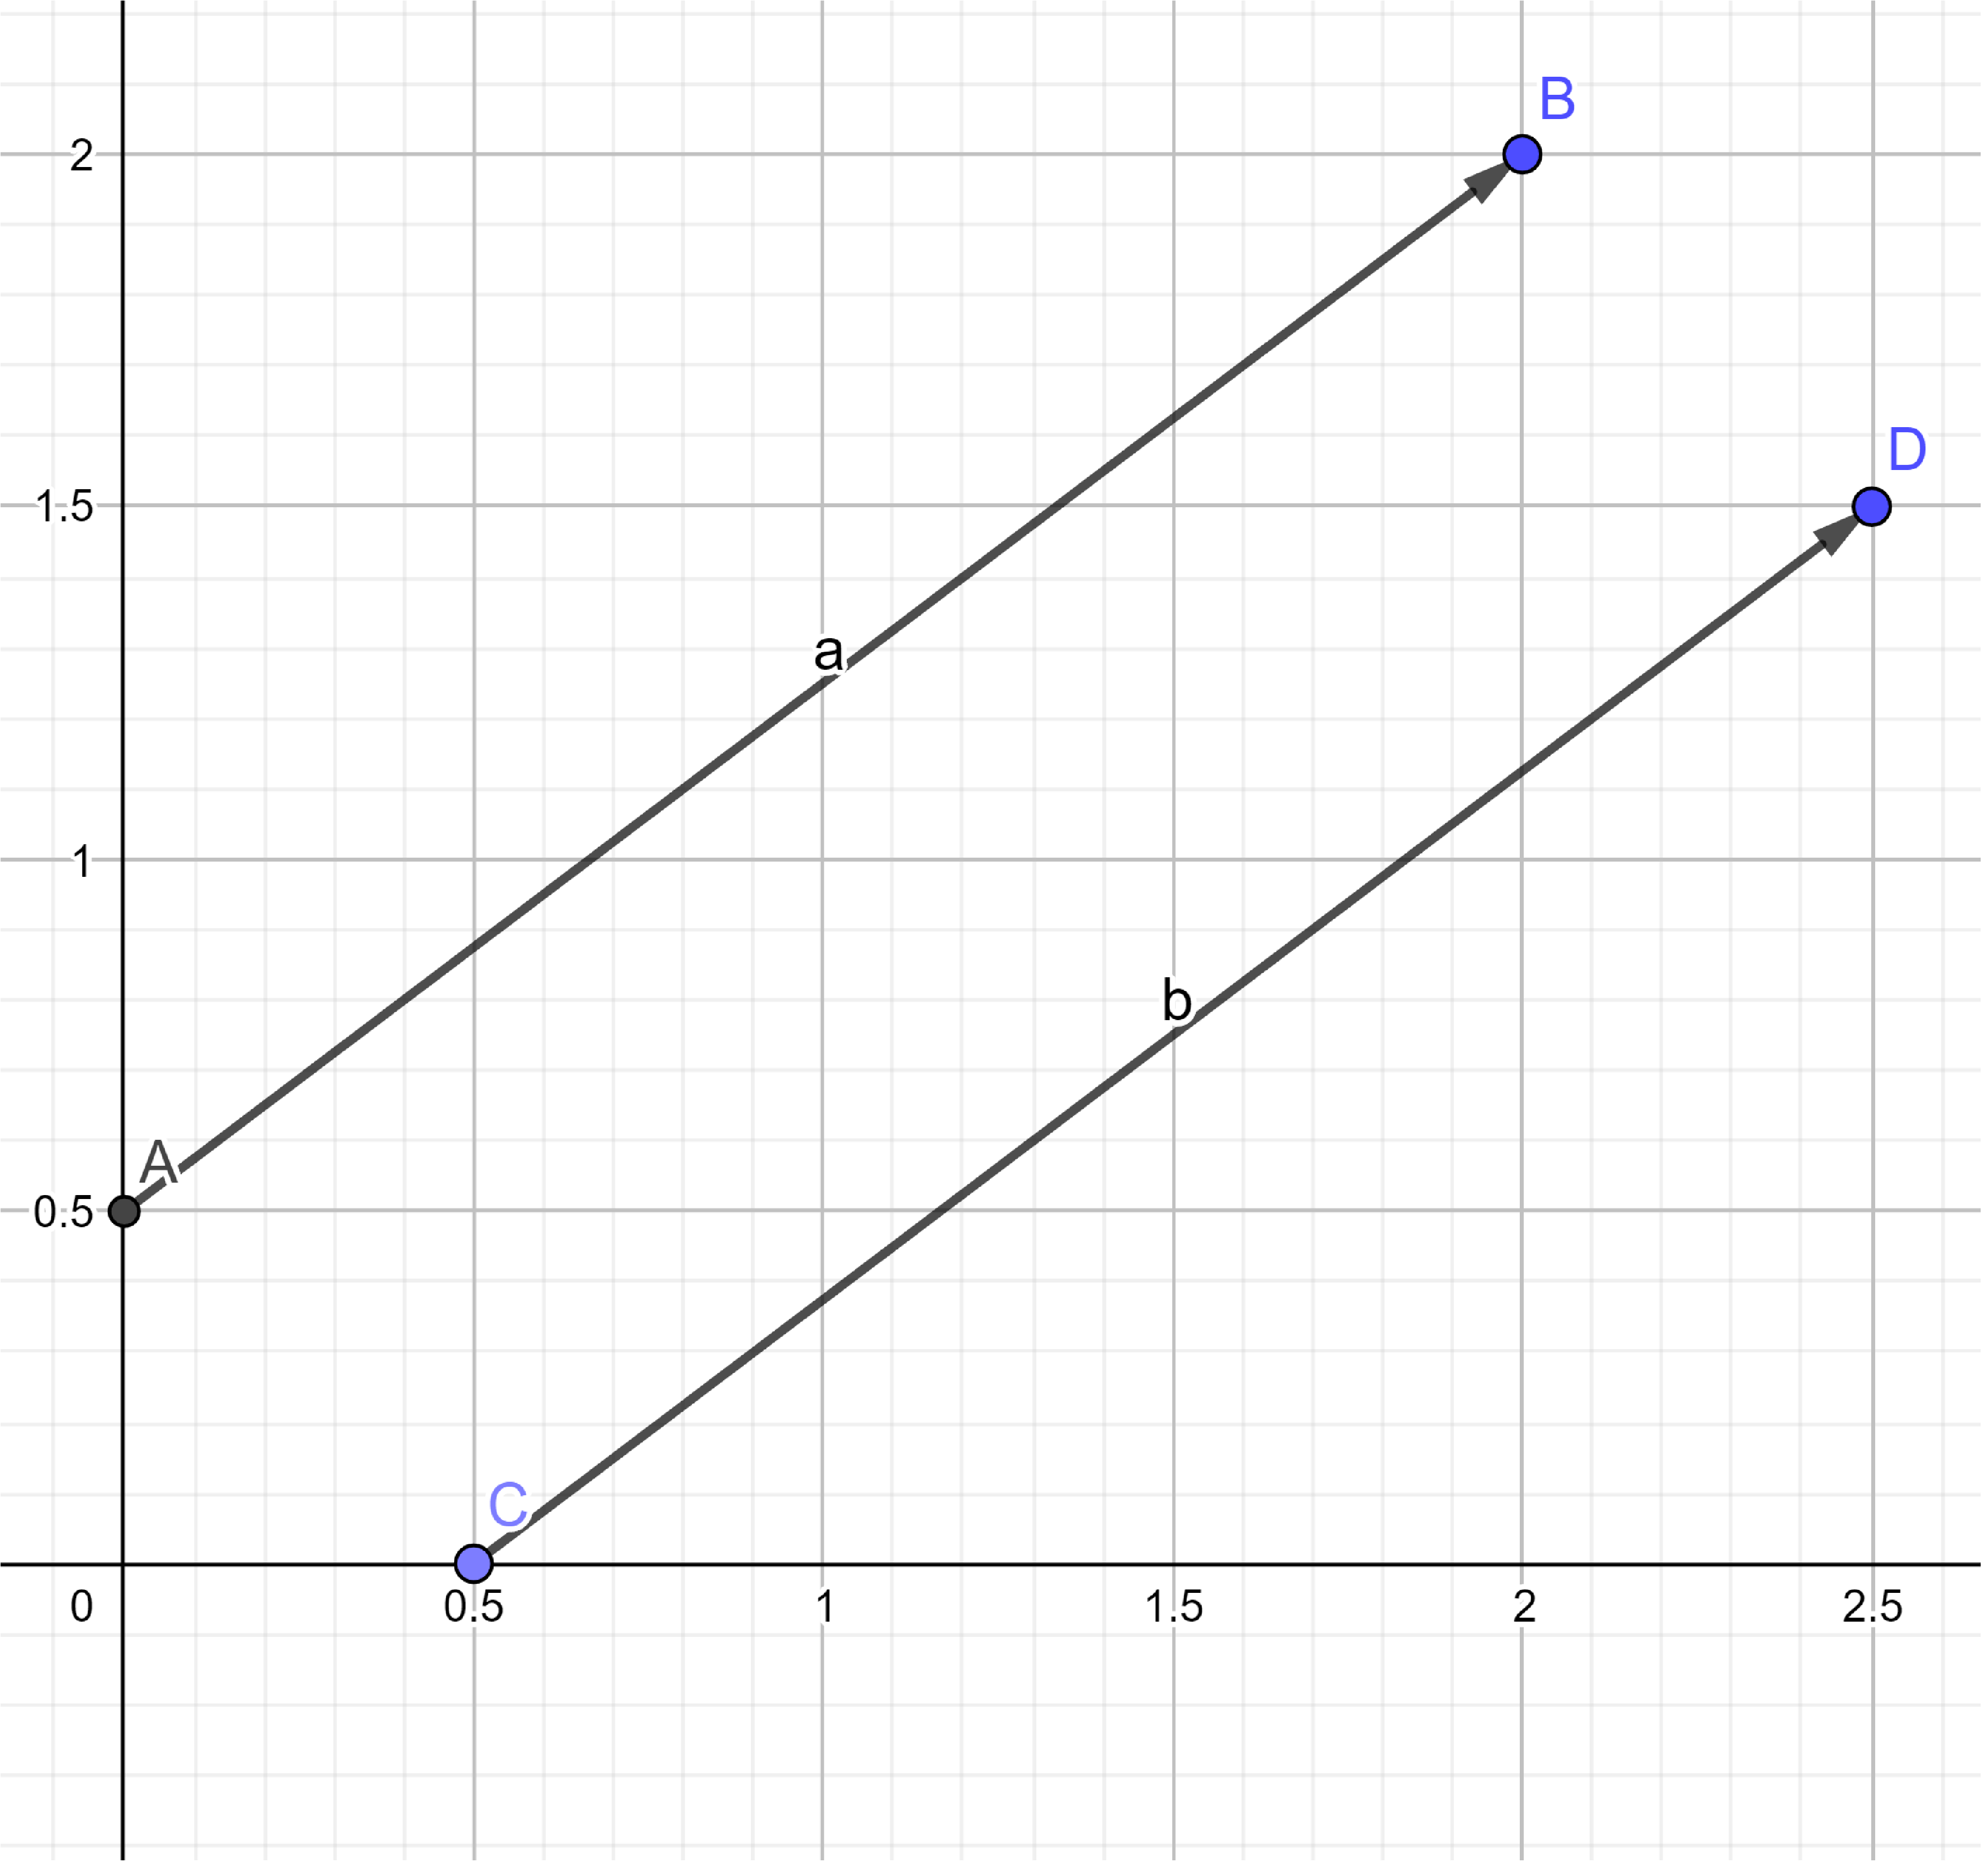
\includegraphics[width=1.3\linewidth]{vect_1} 
	\end{wrapfigure}
	
	Vectors are represented using line segments with arrows to denote their direction. Hence, we may consider vector $\overrightarrow{AB}$.
	
	\begin{itemize}
		\item{Two vectors are s.t.b equal iff they have the same magnitude and act in the same direction.}
		\item{The modulus refers to the size of a vector $\underline{a}$ and is denoted by $\abs{a}$.}
		\item{Two vectors $\underline{a}$ and  $-\underline{a}$  are equal in magnitude but opposite in direction. Hence the negative sign indicates opposing direction.}
		\item{When a vector is multiplied by a scalar, its magnitude changes. thus $\lambda  \underline{a}$ is a vector in the same direction as  $\underline{a}$ but has magnitude $\lambda\abs{\underline{a}}$}
	\end{itemize}
	\section{Position Vectors and Free Vectors}
	\quad When we refer to a vector  $\underline{a}$ we refer to a vector which is not confined to a specific position on the plane or in space.  $\underline{a}$, as such, is a \textit{free vector}.\\
	
	When we refer to the position vector  $\underline{b}$, we refer to a vector which is initially set to start from a specific location, usually, the origin.\\
	\setlength{\columnseprule}{0pt} 
	\begin{multicols}{2}
		\begin{center}
			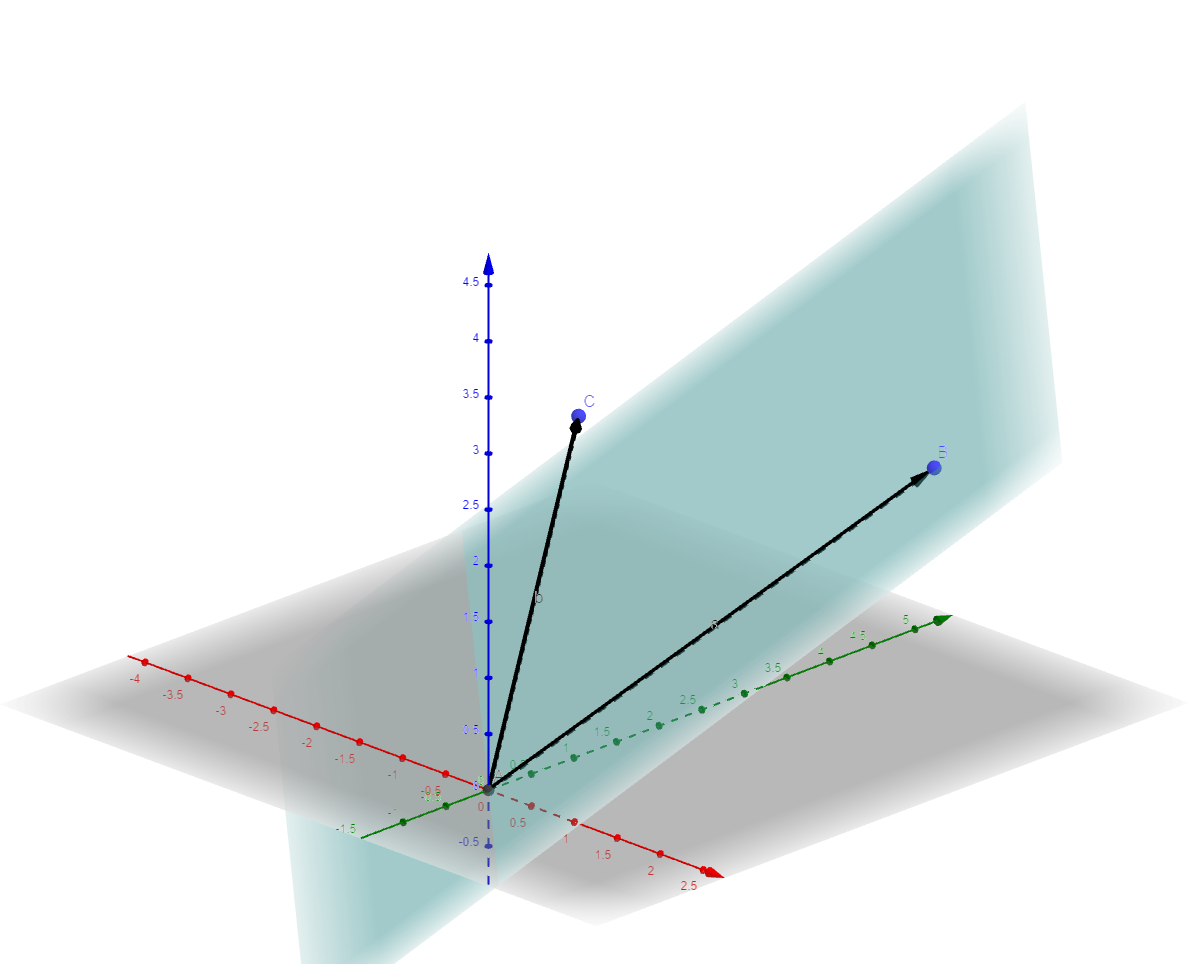
\includegraphics[scale=0.16]{vect_2} 
		\end{center}
		\begin{center}
			~\\~\\~\\
			Suppose that  $\underline{a}$ and  $\underline{b}$ are non-parallel free vectors, and that the origin is a fixed point. There exists only one plane which contains the point $(0,0)$,  $\underline{a}$ and  $\underline{b}$.
		\end{center}
		
	\end{multicols}
	
	Consider another point $p$ on this plane.
	\begin{multicols}{2}
		\begin{center}
			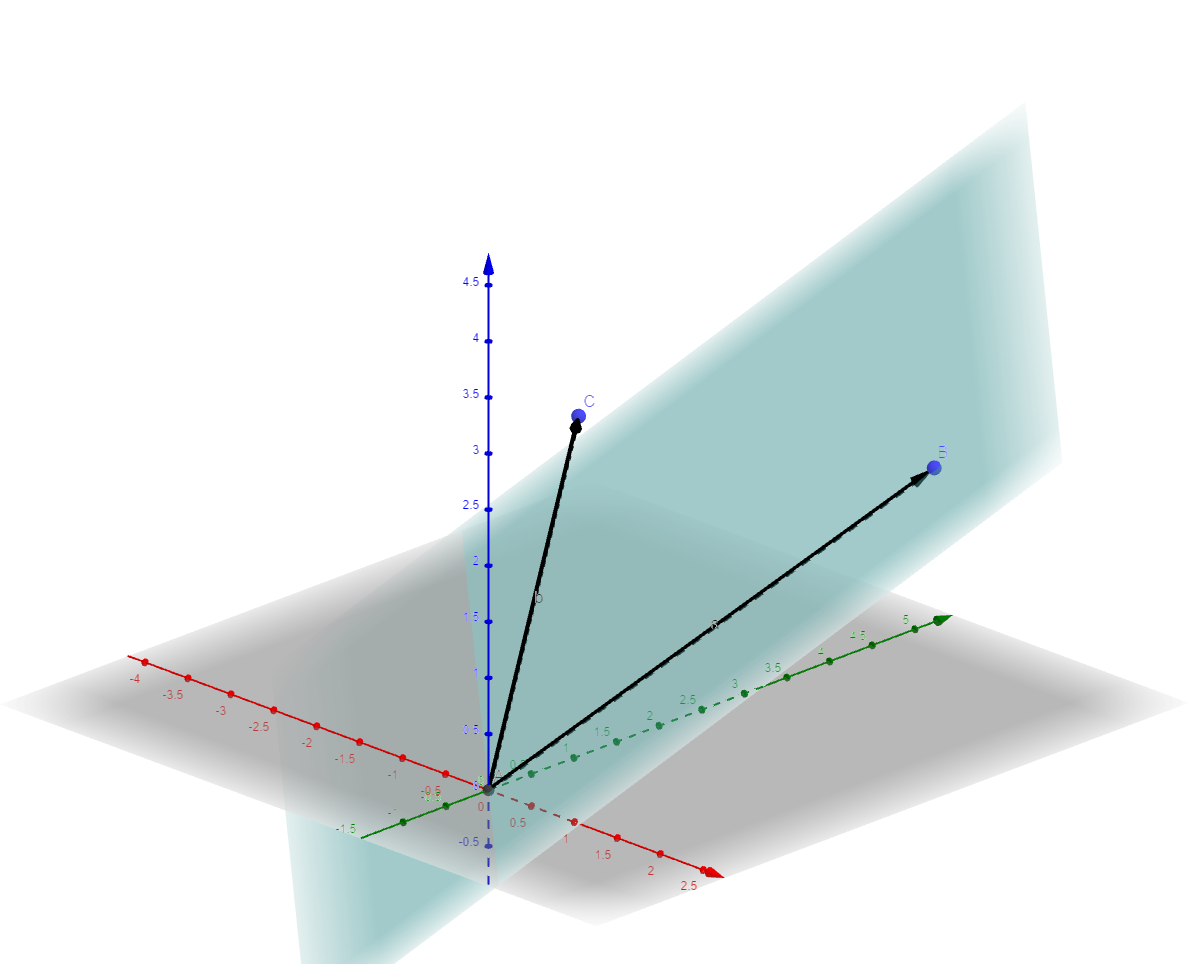
\includegraphics[scale=0.16]{vect_2} 
		\end{center}
		\begin{itemize}
			\item{$\vec{OP}$ is the PV \footnote{Position Vector} of P}
			
			\item{	$\overrightarrow{OC}$ is $\parallel$ to $\textbf{b}$, thus $\overrightarrow{OC} = \lambda \textbf{b}$}
			\item{$\overrightarrow{CP}$ is $\parallel$ to \textbf{a}, thus $\overrightarrow{CP} = \gamma \textbf{a}$}
			\item{$\overrightarrow{OP} = \overrightarrow{OC} + \overrightarrow{PC}	 =\gamma \textbf{a} + \lambda \textbf{b}$}
		\end{itemize}
		
	\end{multicols}
	~\\
	
	Therefore, the point $O$ and the vectors \textbf{a} and \textbf{b} form a frame of reference for the position of any point on the plane. The vectors \textbf{a} and \textbf{b} are known as the base vectors. Any vector parallel to the plane can be expressed in the form $\gamma \textbf{a} + \lambda \textbf{b}$ where $\lambda$ and $\gamma$ are scalar quantities.\\
	
	
	This basis spans the usual $x$ and $y$ plane. The base vectors are \textbf{i} and \textbf{j} respectively denoting the unit base vector in the positive $x$ direction and similarly in the positive $y$ direction.\\
	
	In general, given the points $A(x_1,y_1)$ and $B(x_2,y_2)$, the vector $\overrightarrow{AB}$ is given by:	
	
	
	\begin{center}
		\begin{tcolorbox}[center title,hbox,    %%<<---- here
			lifted shadow={1mm}{-2mm}{3mm}{0.1mm}%
			{black!50!white}]
			\begin{varwidth}{\textwidth}
				\begin{center}
					$$\overrightarrow{AB} = (x_2 -x_1)\textbf{i} - (y_2 -y_1)\textbf{j}$$
					
					$$	\abs{\overrightarrow{AB}} = \sqrt{(x_2 -x_1)^2 + (y_2 -y_1)^2}$$
				\end{center}
			\end{varwidth}
		\end{tcolorbox} 
	\end{center}
	\newpage
	\section{Unit vectors}
	
	
	
	A unit vector is a vector with magnitude 1. Consider vector $\textbf{v}$ \& let $\abs{\textbf{v}}$ be its magnitude. A unit vector in the direction of $\textbf{v}$, denoted by $\hat{\textbf{v}}$ can be obtained by dividing $\textbf{v}$ by its magnitude.
	
	$$\hat{\textbf{v}} = \frac{\textbf{v}}{\abs{\textbf{v}}}$$
	
	
	\section{Vectors in 3D space}
	
	The ideas developed in the previous section can be extended to the 3-dimensional space. Thus any point $A(x_1,y_1,z_1)$ in the 3D space has position vector $\overrightarrow{OA}$.
	\begin{center}
		\begin{tcolorbox}[center title,hbox,    %%<<---- here
			lifted shadow={1mm}{-2mm}{3mm}{0.1mm}%
			{black!50!white}]
			\begin{varwidth}{\textwidth}
				\begin{center}
					$$\overrightarrow{OA} = x\textbf{i} + y\textbf{j} +z\textbf{k}$$
					$$\abs{\overrightarrow{OA} = \sqrt{x^2 + y^2 + z^2}}$$
				\end{center}
			\end{varwidth}
		\end{tcolorbox} 
	\end{center}
	
	Also, given two points $A(x_1,y_1,z_1)$ and $B(x_2,y_2,z_2)$, the vector $\overrightarrow{AB}$ is given by:
	\begin{center}
		\begin{tcolorbox}[center title,hbox,    %%<<---- here
			lifted shadow={1mm}{-2mm}{3mm}{0.1mm}%
			{black!50!white}]
			\begin{varwidth}{\textwidth}
				\begin{center}
					$$\overrightarrow{AB} = (x_2 -x_1)\textbf{i} - (y_2 -y_1)\textbf{j} + (z_2 - z_1)\textbf{k}$$
					
					$$	\abs{\overrightarrow{AB}} = \sqrt{(x_2 -x_1)^2 + (y_2 -y_1)^2 + (z_2 - z_1)^2}$$
				\end{center}
			\end{varwidth}
		\end{tcolorbox} 
	\end{center}
	
	\subsection{Direction ratios of a Vector}
	
	Given the vector $a\textbf{i}+b\textbf{j}+c\textbf{k}$, the ratios $a\colon b\colon c$ are called the direction ratios of the vector.\\
	
	Since the numbers $a$, $b$ and $c$ define the inclination of the vector in space, it follows that parallel vectors have equivalent direction vectors.\\
	
	In vectors, parallelism can be of two types:\\
	\begin{itemize}
		\item{Like parallel}
		\subitem{Two like parallel vectors both travel in the same direction.}
		\item{Unlike parallel}
		\subitem{Two unlike parallel vectors are still positionally parallel but act in the opposite direction.}
	\end{itemize}
	~\\
	In both cases, the direction ratios, however, are the same. For instance, consider the two vectors:
	
	\begin{alignat*}{2}
		&   & \textbf{a} & = 3\textbf{i} + 5\textbf{j} + 6\textbf{k}  \\
		&   & \textbf{b} & = -3\textbf{i} -5\textbf{j}  - 6\textbf{k} 
	\end{alignat*}
	Both of them will simplify to an equivalent ratio when multiplied by $-1$.
	
	\subsection{3-Dimensional Lines}
	
	Lines in 3D are better explained through vector geometry. Coordinate geometry is sufficient for the analysis of lines in 2D, however, when adding the third dimension, this becomes inefficient.
	
	\subsubsection{Equation of a straight line}
	
	The previous notion of the definition of a straight line, $y=mx+c$ or more particularly $y_2-y_1 = m(x_2-x_1)$ becomes insufficient to define a line on 3 planes of space.\\
	
	A line in 3D space is defined by a point through which it passes, and a direction to which it is parallel. Consider the following diagram:
	
	
	\begin{center}
		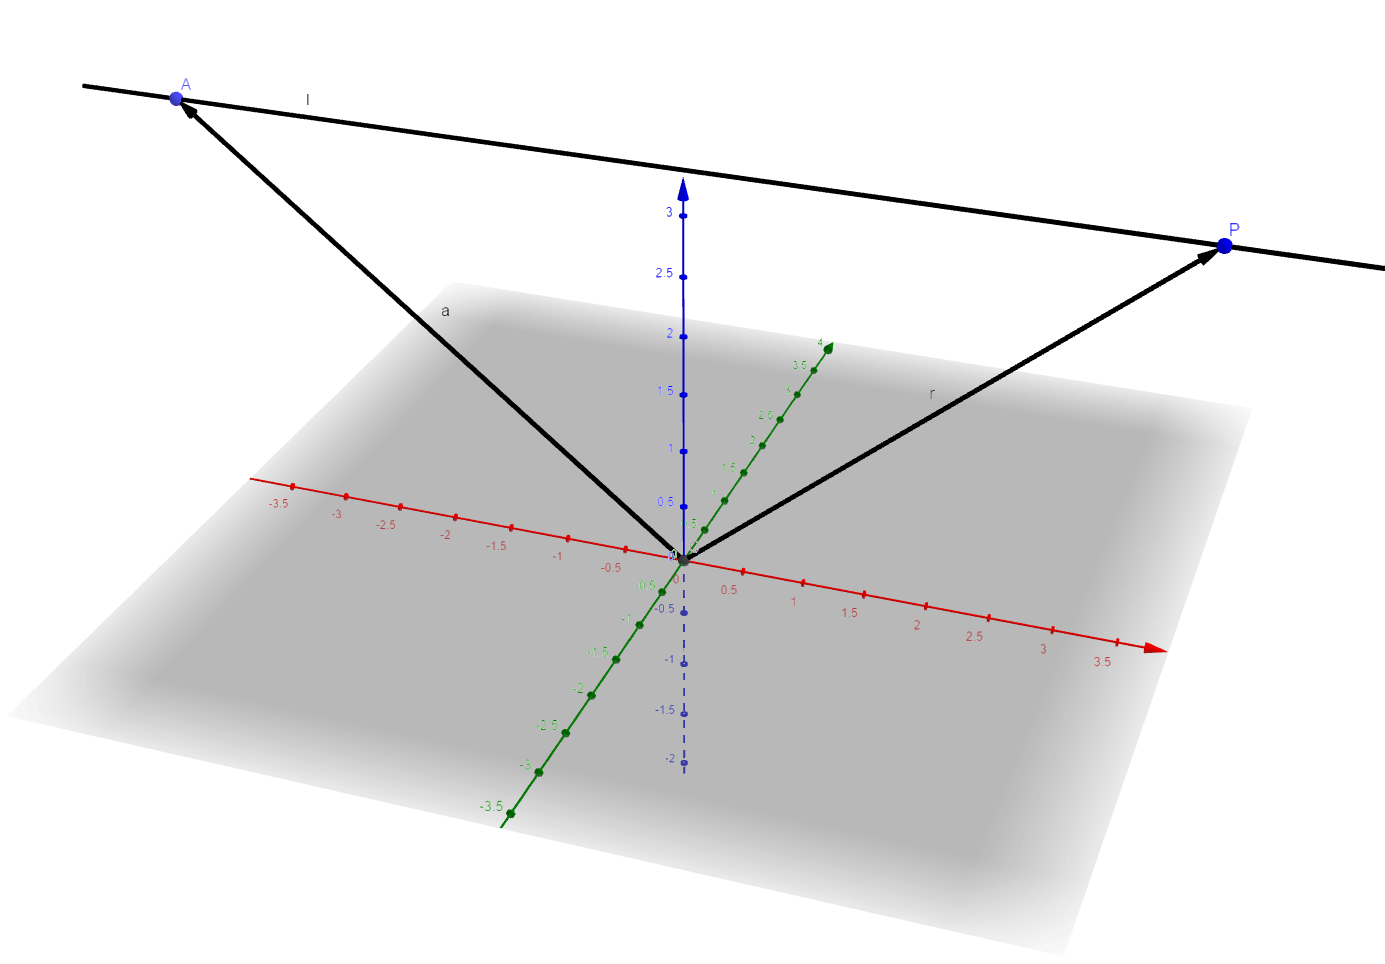
\includegraphics[scale=0.15]{vect_3}
	\end{center}
	
	
	Let $A$ be a fixed point on the line $l$ with position vector $\textbf{a}$ \& let $P$ represent a general point on the line. Let the position vector of $P$ be $\textbf{r}$. Consider also a vector $\textbf{m}$ parallel to the line $l$.\\
	
	We need to find the equation of line $l$, specifically, a rule defining the line $l$ which governs all points $P$ on this line. To generate the line $l$ as described above, the point $P$ must be such that $\overrightarrow{AP}$ is parallel to $\textbf{m}$.
	
	\begin{multicols}{3}
		$$	 \textbf{r}  = \textbf{a} + \lambda \textbf{m}$$
		
		\begin{alignat*}{2}
			&   & x & = x_1 + \lambda a \\
			&   & y & = y_1 + \lambda b \\
			&   & z & = z_1 + \lambda c 
		\end{alignat*}
		\begin{alignat*}{2}
			&   & x & = x_1 + \lambda a \\
			&   & y & = y_1 + \lambda b \\
			&   & z & = z_1 + \lambda c 
		\end{alignat*}
		\begin{center}
			~\\
			~\\
			$\frac{x-x_1}{a} = \frac{y-y_1}{b} = \frac{z-z_1}{c}$
		\end{center}
	\end{multicols}
	\end{document}
		%\documentclass{standalone}
\begin{document}
	\chapter{Inequalities}
	\section{Quadratic Inequalities}
	\begin{example}
		Solve the inequality $x^2-2x>3$
	\end{example}
	
	\begin{center}
		$$x^2-2x>3$$
		$$\implies x^2-2x-3>0$$
		$$\text{Let }x^2-2x-3=0$$
		$$\implies(x-3)(x+1)=0$$
	\end{center}	
	\begin{center}
		\begin{tikzpicture}
			\begin{axis}[
				width=8cm,
				height=6cm,
				axis line style={-},
				xmin=-4,
				xmax=4,
				ymin=-4,
				ymax=5,
				xtick={-1,3}, % remove all ticks from x-axis
				ytick={-3}, % ditto for y-axis
				xlabel=$x$, 
				ylabel=$y$,
				axis lines=center, % default is to make a box around the axis
				samples=100]
				\addplot [black] {x^2 - 2*x - 3}
				;
			\end{axis}
		\end{tikzpicture}
	\end{center}
	\hrulefill
	\begin{example}
		Solve the inequality $\quad \dfrac{2x^2}{5} \leq \dfrac{7x+10}{2}$
	\end{example}
	\begin{center}
		$$4x^2 \leq 35x + 50$$
		$$\implies 4x^2-35x-50\leq 0$$
		$$\text{Let }\quad 4x^2-35x-50=0$$
		$$(4x+5)(x-10)=0$$
		\begin{tikzpicture}
			\begin{axis}[
				width=8cm,
				height=6cm,
				axis line style={-},
				xmin=-2,
				xmax=11,
				ymin=-127,
				ymax=50,
				xtick={-5/4,10}, 
				ytick={-50}, 
				xlabel=$x$, 
				ylabel=$y$,
				axis lines=center, 
				samples=100]
				\addplot [black] coordinates{
					(-1,-17)(0,-48)(1,-79)(2,-110)(3,-141)(4,-172)(5,-203)(6,-234)(7,-265)(8,-296)(9,-327)(10,-358)(11,-389)	
				};
			\end{axis}
		\end{tikzpicture}
	\end{center}
	
	\hrulefill
	\end{document}
		\documentclass{standalone}


\begin{document}
	
	\chapter{Series}
	
	\section{Sequences}
	
	Consider the following set of numbers: 
	\begin{center}
		$2,4,6,8,...$\\
		$1,2,4,8,16,...$\\
		$4,9,16,25,...$\\
	\end{center}
	In each of the above cases, the numbers are written in a particular order and there is a clear rule for obtaining the next number and as many numbers in the list.\\
	
	The above are all examples of sequences where a sequence is a set of terms in a defined order with a rule for obtaining the terms.
	
	\section{Summation Series}
	
	When the terms of a sequence are added, a summation series is formed:
	
	\begin{multicols}{2}
		\begin{center}
			$2+4+6+8+10+...$\\
			$1+2+4+8+16+...$\\
			$4+9+16+25+36+...$\\
		\end{center}
		\begin{center}
			~\\
			are all examples of series.
			~\\
		\end{center}
	\end{multicols}
	A series can be finite or infinite, where a finite series consists of a fixed number of terms, whereas an infinite series has an infinite number of terms.\\
	
	Considering the follwing series, \[1+\frac{1}{2}+ \frac{1}{4}+\frac{1}{8}+\frac{1}{16}+...\] we can notice that the general term of this series is $\frac{1}{2^r}$. The general term of a series is not unique, it depends on the initial value of $r$. Thus, the general term $\frac{1}{2^{r-1}}$ also corresponds to the above series but we take the initial value of $r$ to be 1.\\
	
	A summation series can be defined in a concise way using the Greek letter $\Sigma$ denoting the \textit{summation of terms}. The above series may be expressed as \[\sum_{r=0}^\infty \frac{1}{2^r}\] which is equivalent to \[\sum_{r=1}^\infty \frac{1}{2^{r-1}} \quad r \in \mathbb{Z}\]
	
	\section{Arithmetic Progressions}
	\subsection{Definition}
	An arithmetic progression is a sequence of numbers starting with term $a$, in which successive terms are obtained by adding the same constant, denoted by $d$, reffered to as the \textbf{common difference}.\\
	
	\subsection{General term}
	Let us consider the general A.P with first term $a$ and common difference $d\colon$ \[a+(a+d)+(a+2d)+(a+3d)+(a+4d)+(a+5d)+...\] By observing the coefficient of $d$ and the position of the term, we can conclude that the general term can be obtained by the equation: \[T_n = a+(n-1)d\]
	\subsection{Sum of the first n terms}
	Considering an A.P. with $n$ terms, let the first term be $a$, the common difference to be $d$	and the last term to be $l$
	
	\begin{align*}
				S_n &= a+(a+d)+(a+2d)+(a+3d)+(a+4d)+(a+5d)+...+(l-d)+l\\
\implies	S_n &= l+(l-d)+(l-2d)+(l-3d)+(l-4d)+(l-5d)+...+(a+d)+a\\
	\implies	2S_n &= n(2a+l)\\
 \implies   S_n  &= \frac n2 (2a+l)\\
	   		&= \frac n2 (2a +(n-1)d)
	\end{align*}
	\newpage
	\section{Geometric progressions}
	\subsection{Definition}
	A geometric progression is a sequence of numbers starting with term $a$, in which successive terms are obtained by multiplying the same constant, denoted by $r$, reffered to as the \textbf{common ratio}.\\
	
	\subsection{General term}
	
	Let us consider a general G.P. with first tirm $a$ and a common ratio $r$: \[a+ar+ar^2+ar^3+ar^4+ar^5+...+ar^n-1+\ldots\]
	By observing the exponent of $r$ and the position of the term we can conclude that the general term can be obtained by the equation: \[\mathrm{T_n} = ar^{n-1}\]
	
	\subsection{Sum of the first n terms}
	Considering a G.P. with first term $a$, common ratio $d$ and it's sum denoted by $S_n$:
	
	\begin{align*}
		S_n = a+&ar+ar^2+ar^3+ar^4+ar^5+\ldots+ar^{n-1}+\ldots\\
		rS_n = \phantom{a+}&ar+ar^2+ar^3+ar^4+ar^5+\ldots+ar^n+\ldots\\
		S_n - rS_n =\phantom{a+}& a-ar^n\\
		(1-r)S_n = \phantom{a+}&a(1-r^n)\\
		S_n = \phantom{a+}&  \frac{a(1-r^n)}{1-r} \qed
		\end{align*}
	
	
	\section{Convergence of a series}
	
	For any\footnote{A.P's by definition \textbf{do not} converge.} given G.P., we can always add infinitely many times more terms to the end of the series, but what hapens to it's sum? Given that $\abs r = 1$, the sum will always get infinitesimally closer to a definite number.\\
	
	Considering the G.P. $\frac 12 + \frac 14 + \frac 18 + \frac 1 {16} + \ldots$ we can observe that if you keep on adding terms and summing them, the sum will approach 1. In mathematical language we say \[\text{as } n \rightarrow \infty\,,\,S_n = 1\] or \[\lim_{n\to\infty}S_n = 1\]
	
	\section{Binomial theorem}
	
	The binomial theorem states that \[(x+y)^n = \sum_{k=0}^n\begin{pmatrix}n\\k\end{pmatrix} x^ky^{n-k}	\]
	
	\section{Maclaurin Series}
	\subsection{Derivation}
	Let $f(x)$ be nay function of $ x $ and suppose that $ f(x) $ can be expanded as a series of ascending powers of $ x $ and that this series can be differentiated $ w.r.t. x $
	\begin{center}
		$	f(x) \equiv a_0   + a_{1}x  + a_{2}x^2 + a_{3}x^3 + a_{4}x^4 + ... +	 a_{r}x^r$\\
		\text{where $a_n$ are constants to be found}
	\end{center}
	Thus, inputting $0$ into $f(x)$ returns:
	$$\boxed{f(0) = a_{0}}$$\\
	Differentiating  $f(x)$ $w.r.t.x\colon$ 
	$$f'(x) \equiv a_{1} + 2a_{2}x + 3a_{3}x^2 + 4a_4x^3 + \cdots + ra_{r}x^{r-1} + \cdots$$
	Inputting $0$ into $f'(x)\colon$
	$$\boxed{f'(0) = a_1}$$\\
	Differentiating $f'(x)$ $w.r.t.x\colon$
	$$f''(x) \equiv 2a_{2} + 6a_{3}x + 12a_4x^2 + \cdots + (r-1)(r)a_{r}x^{r-2} + \cdots$$
	Inputting $0$ into $f''(x)\colon$
	$$\boxed{f''(0) = 2a_2}$$\\
	Differentiating $f''(x)$ $w.r.t.x\colon$
	$$f'''(x) \equiv 6a_{3} +24a_4x + \cdots + (r-2)(r-1)(r)a_{r}x^{r-3}+ \cdots$$
	Inputting $0$ into $f'''(x)\colon$
	$$\boxed{f'''(0) = (2)(3)a_3}$$
	$$\vdots$$
	\newpage
	By the above calculation we can conclude that: 
	$$\boxed{a_r = \frac{f^r(x)}{r!}}$$
	Considering all of the above: 
	
	\tcbset{
		enhanced,
		colback=red!5!white,
		boxrule=0.1pt,
		colframe=black!75!black,
		fonttitle=\bfseries
	}
	\begin{center}
		\begin{tcolorbox}[center title,hbox,    %%<<---- here
			lifted shadow={1mm}{-2mm}{3mm}{0.1mm}%
			{black!50!white}]
			\begin{varwidth}{\textwidth}
				\begin{center}
					$f(x) \equiv f(0) + f'(0)x + \dfrac{f''(0)x^2}{2!} + \dfrac{f'''(0)x^3}{3!} + \cdots + \dfrac{f^r(0)x^r}{r!} + \cdots$\\
					\bigskip
					$\displaystyle \therefore \quad f(x) \equiv \sum_{r=1}^{\infty} \dfrac{f^r(x)}{r!}$
				\end{center}
			\end{varwidth}
		\end{tcolorbox} 
	\end{center}
	
	
	This is known as Maclaurin's Theorem, and can be obtained if and only if $f^r(0) \in \mathbb{R}$. In the following examples we use Maclaurin's Theorem to obtain the series expansion of some standard equations. The range of validity of each expansion is left as an exercise to the reader.
	\subsection{Examples}
	\begin{example}
		\emph{Express} $e^x$ \emph{as a series expansion using the Maclaurin theorem.}
	\end{example}
	Let $f(x) = e^x$
	\begin{alignat*}{5}
		&   & f(x)    & = & e^x \quad & \Rightarrow\quad & f(0) = 1    \\
		&   & f'(x)   & = & e^x \quad & \Rightarrow\quad & f'(0) = 1   \\
		&   & f''(x)  & = & e^x \quad & \Rightarrow\quad & f''(0) = 1  \\
		&   & f'''(x) & = & e^x \quad & \Rightarrow\quad & f'''(0) = 1 
	\end{alignat*}
	
	$$\therefore \quad e^x  = 1 + x + \frac{x^2}{2!} + \frac{x^3}{3!} + \frac{x^4}{4!} +\ldots + \frac{x^r}{r!} + \ldots $$
	\hrulefill
	\begin{example}
		\emph{Express} $\cos x$ \emph{as a series expansion using the Maclaurin theorem.}
	\end{example}
	\begin{alignat*}{5}
		&   & f(x)    & =           & \cos (x) \quad & \Rightarrow\quad & f(0) = 1    \\
		&   & f'(x)   & = \text{ -} & \sin (x) \quad & \Rightarrow\quad & f'(0) = 1   \\
		&   & f''(x)  & = \text{ -} & \cos(x) \quad  & \Rightarrow\quad & f''(0) = 1  \\
		&   & f'''(x) & =           & \sin (x) \quad & \Rightarrow\quad & f'''(0) = 1 
	\end{alignat*}
	$$\therefore \quad \cos (x)  = 1 - \frac{x^2}{2!} + \frac{x^4}{4!} -\frac{x^6}{6!}+\ldots + (-1)^r\times\frac{x^{2r}}{2r!} + \ldots $$\\
	The above expansion justifies the fact that when $x$ is very small and thus high powers of $x$ may be neglected, then: \boxed{\cos x \approx 1- \frac{x^2}{2}}\\
	\begin{example}
		\emph{Express} $\ln(1+x)$ \emph{as a series expansion using the Maclaurin theorem.}
	\end{example}
	
	\begin{alignat*}{5}
		&   & f(x)    & = & \ln(1+x)      \quad & \Rightarrow  \quad & f(0)    & = 0  \\
		&   & f'(x)   & = & (x+1)^{-1} \quad    & \Rightarrow  \quad & f'(0)   & = 1  \\
		&   & f''(x)  & = & -(1+x)^{-2}  \quad  & \Rightarrow \quad  & f''(0)  & = -1 \\
		&   & f'''(x) & = & 2(1+x)^{-3} \quad   & \Rightarrow  \quad & f'''(0) & = 2  
	\end{alignat*}
	$$\therefore \quad \ln(1+x)  = x - \frac{x^2}{2} + \frac{x^3}{3} - \ldots + (-1)^{r+1}\times\frac{x^r}{r} + \ldots $$\\
	\hrulefill
	
	\begin{example}
		\emph{Expand} $\arcsin(x)$ \emph{up to the term in $x^3$. By putting $x=\frac{1}{2}$, find an approximate value for $\pi$}
	\end{example}
	
	\begin{alignat*}{5}
		& f(x)    & = & \arcsin(x)      \quad                                   & \Rightarrow  \quad & f(0)    & = 0 \\
		& f'(x)   & = & (1-x^2)^{\frac{-1}{2}} \quad                            & \Rightarrow  \quad & f'(0)   & = 1 \\
		& f''(x)  & = & x(1-x^2)^{\frac{-3}{2}}\quad                            & \Rightarrow \quad  & f''(0)  & = 0 \\
		& f'''(x) & = & 3x(1-x^2)^{\frac{-5}{2}} + (1-x^2)^{\frac{-3}{2}} \quad & \Rightarrow  \quad & f'''(0) & = 1 
	\end{alignat*}
	$$\therefore \quad \arcsin(x)   = x + \frac{x^3}{3!} + \ldots $$\\
	Putting $x = \frac{1}{2}$\\
	\begin{alignat*}{2}
		&          & f\left(\frac{1}{2}\right) & = \frac{\pi}{6}                                \\
		& \implies & \pi                       & \approx 6\left(\frac{1}{2}+\frac{1}{81}\right) \\
		& \implies & \pi                       & \approx \frac{83}{27}                          
	\end{alignat*}
	\newpage
	\subsection{Expanding compound functions using standard functions}
	\begin{example}
		Expand $a)\quad \dfrac{e^{2x}+ e^{-3x}}{e^x}\quad b)\quad \ln\left( \dfrac{1-2x}{(1+2x)^2}\right)  $as series of ascending powers of $x$ up to the term in $x^4$. Give the general term in each case and the range of values of $x$ for which each expansion is valid.
	\end{example}
	\begin{alignat*}{2}
		a) &                  & e^x                                    & = 1 + x + \frac{x^2}{2!} + \frac{x^3}{3!} + \frac{x^4}{4!} +\ldots                                                                                                  \\
		&                  & e^{-3x}                                & = 1 + (-3)x + \frac{(-3x)^2}{2!} + \frac{(-3x)^3}{3!} + \frac{(-3x)^4}{4!} +\ldots                                                                                  \\
		& \therefore \quad & e^{x} + e^{-3x}                        & = \left (1 + x + \frac{x^2}{2!} + \frac{x^3}{3!} + \frac{x^4}{4!}\right ) + \left (1 + (-3)x + \frac{(-3x)^2}{2!} + \frac{(-3x)^3}{3!} + \frac{(-3x)^4}{4!}\right ) \\
		&                  &                                        & = 2 -2x + \frac{10x^2}{2!} - \frac{26x^3}{3!} + \frac{89x^4}{4!}                                                                                                    \\
		\bigskip\\
		b) &                  & \ln\left(\dfrac{1-2x}{(1+2x)^2}\right) & = \ln(1-2x) -2\left (\ln(1+2x)\right)                                                                                                                               
		\intertext{\emph{Consider $\ln(1-2x)\colon$}}
		&                  & \ln\left(1+(-2x)\right)                & = -2x + -2x^2-\frac{8x^3}{3}-4x^4 + \ldots + \frac{(-1)^{r-1}(-2x)^r}{r}+ \ldots                                                                                    \\
		\intertext{\emph{Consider $\ln(1+2x)\colon$}}
		&                  & \ln\left(1+2x\right)                   & = 2x + -2x^2+\frac{8x^3}{3}-4x^4 +\ldots + \frac{-2(-1)^{r-1}(2x)^r}{r} + \ldots                                                                                    \\ 
		& \therefore       & \ln\left(\dfrac{1-2x}{(1+2x)^2}\right) & = \left( -2x + -2x^2-\frac{8x^3}{3}-4x^4\right) -2\left(2x + -2x^2+\frac{8x^3}{3}-4x^4\right)                                                                       \\
		&                  &                                        & = -6x+2x^2-8x^3	+4x^{4}                                                                                                                                             \\
	\end{alignat*}
	\text{Range of Validity:}
	\begin{multicols}{2}
		\begin{center}
			$$	\quad\frac{(-1)^{r-1}(-2x)^r}{r} - \frac{2(-1)^{r-1}(2x)^r}{r}$$\\
			$$  =\frac{(-1)^{r-1}(-1)^r(2x)^r+2(-1)^r(2x)^r}{r}$$\\
			$$	=\frac{(-1)^{2r-1}(2x)+2(-1)^r(2x)^r}{r}$$\\
			$$	=\frac{\left( (-1)^{2r-1}+2(-1)^r\right) (2x)^r}{r}$$\\
			$$  =\frac{ \left(-1+2(-1)^r\right(2x)^r)}{r}$$
			$$ =\frac{2^r(2(-1)^r -1)x^r}{r}$$							
		\end{center}
	\end{multicols}
	
	\begin{example}
		Expand  $\ln\left(\frac{x+1}{x}\right)\quad$as series of ascending powers of $x$ up to the term in $x^4$. Give the general term in each case and the range of values of $x$ for which each expansion is valid.
	\end{example}
	
	$$f(x) \ln\left(\frac{x+1}{x}\right)  = \ln\left(1+\frac{1}{x}\right ) $$
	
	\begin{alignat*}{5}
		&   & f(x)    & = & \ln(1+\frac{1}{x})    \quad & \Rightarrow  \quad & f(0)    & = 0  \\
		&   & f'(x)   & = & (x+1)^{-1} \quad            & \Rightarrow  \quad & f'(0)   & = 1  \\
		&   & f''(x)  & = & -(1+x)^{-2}  \quad          & \Rightarrow \quad  & f''(0)  & = -1 \\
		&   & f'''(x) & = & 2(1+x)^{-3} \quad           & \Rightarrow  \quad & f'''(0) & = 2  
	\end{alignat*}
	
	\begin{center}
		$=\frac{1}{x} - \frac{1}{2x^2} + \frac{1}{3x^3} - \frac{1}{4x^4} + \ldots + \frac{(-1)^{r+1}}{r} $
	\end{center}
	\hrulefill
	\begin{example}
		Expand $\sin^2{x}$ using Maclaurin's series up to $x^4$
	\end{example}
	\bigskip
	$$sin^2(x)\equiv\frac{1-\cos(2x)}{2}$$
	\begin{alignat*}{2}
		\intertext{\emph{Consider} $\cos(2x)\colon$} &                 &           & =1-\frac{(2x)^{2}}{2!} + \frac{(2x)^4}{4!}  - \cdots + \frac{(-1)^r(2x)^{2r}}{(2r)!}+\cdots           \\
		&                 &           & =1-2x^2+\frac{2x^4}{3}-\cdots+\frac{(-1)^r(2x)^{2r}}{(2r)!}+\cdots                                    \\
		& \therefore\quad & \sin^2(x) & \equiv \frac{1}{2}\left( 1-(1-2x^2+\frac{2x^4}{3}-\cdots+\frac{(-1)^r(2x)^{2r}}{(2r)!}+\cdots)\right) \\
		&                 &           & =\frac{1}{2}\left(1-1+2x^2 - \frac{2x^4}{3} +\cdots+\frac{(-1)^r(2x)^{2r}}{(2r)!}+\cdots\right)       \\
		&                 &           & =x^2-\frac{x^4}{3} +\cdots+\frac{(-1)^{r+1}(2x)^{2r}}{(2r)!}+\cdots                                   
	\end{alignat*}
	\newpage
	\begin{example}
		Given $e^{2x}\cdot \ln{1+ax}$ find possible values for $p$ and $q$.
	\end{example}
	\begin{alignat*}{2}
		\intertext{\emph{Consider} $e^{2x}\colon$}
		&                 & e^{2x}                & = 1+2x + \frac{(2x)^2}{2!} + \frac{(2x)^{3}}{3!} +\cdots +  \frac{x^r}{r!} + \cdots           \\
		\intertext{\emph{Consider} $\ln(1+ax)\colon$}
		&                 & \ln(1+ax)             & = ax - \frac{(ax)^2}{2} + \frac{(ax)^3}{3} - \cdots + \frac{(-1)^{r+1}x^r}{r} + \cdots        \\
		& \therefore\quad & e^{2x}\cdot \ln(1+ax) & = \left(1+2x+2x^2+\frac{4x^3}{3}\right) \left(ax - \frac{a^2x^2}{2} + \frac{a^3x^3}{3}\right) \\
		&                 &                       & =ax-\frac{a^2x^2}{2}+\frac{a^3x^3}{3}+2ax^2-2a^2x^3                                           \\
		&                 &                       & =ax-\left(\frac{a^2}{2}+2a\right) x^2+\left( \frac{a^3}{3}-2a^2\right) x^3                    
	\end{alignat*}
	~\\
	\begin{equation*}
		\therefore\left.
		\begin{alignedat}{2}
			\hspace{0.5 in}	&&p&=a\\
			&&	\frac{a^2}{2}+2a&=\frac{-3}{2}\\
			&&	\frac{a^3}{3}-2a^2&=q
		\end{alignedat}	\right\}
	\end{equation*}
	
	\begin{center}
		$$ p = -3,-1 $$
		$$ q= -27, -\dfrac{7}{3}$$
	\end{center}
	\hrulefill
	\newpage
	\section{Summation of Series}
	\subsection{Method 1: Generating differences}
	
	\begin{example}
		Simplify $f(r)-f(r+1)$, when $f(x) = \frac{1}{r^2}$. Hence, find the sum up to $n$ terms of:\\ $$\sigma_1 = \frac{3}{1^2\cdot 2^2} + \frac{5}{2^2\cdot 3^2} + \frac{7}{3^2\cdot 4^2} + \ldots$$
	\end{example}
	~\\
	Simplifying $f(r) - f(r+1)\colon$
	\begin{alignat*}{2}
		&   & f(r)-f(r+1) & = \frac{1}{r^{2}} - \frac{1}{(r+1)^{2}} \\
		&   &             & =\frac{(r+1)^{2}-r^2}{r^2(r+1)^{2}}     \\
		&   &             & =\frac{2r+1}{r^2(r+1)^2}                
	\end{alignat*}
	\textit{Generating series and adding}\\
	\textit{quantitatively equivalent terms:}
	\begin{center}
		$	\frac{1}{1^2} - \cancel{\frac{1}{2^2}}$
		$$	\cancel{\frac{1}{2^2}} - \cancel{\frac{1}{3^2}}$$
		$$	\cancel{\frac{1}{3^2}} - \cancel{\frac{1}{4^2}}$$
		$$\vdots$$
		$$\cancel{\frac{1}{n^2}} - \frac{1}{n+1^2}$$
		~\\
		$$\boxed{\therefore \quad \sigma_1 = 1 - \frac{1}{n+1^2}}$$
	\end{center}
	\hrulefill
	\begin{example}
		If $f(r) = r(r+1)!$ simplify $f(r) - f(r-1)$. Hence sum the series:\\
	\end{example}
	\begin{center}
		$\sigma_1 = 5\cdot 2! + 10\cdot 3! + 17\cdot 4! +  ... + (n^2=1)n!$\\
	\end{center}
	\hrulefill
	\begin{alignat*}{2}
		&   & f(r)-f(r-1) & =r(r+1)! - (r-1)r!  \\
		&   &             & =r(r+1)r! - (r-1)r! \\
		&   &             & =r!(r^2+r-r+1)      \\
		&   &             & =r!(r^2+1)          
	\end{alignat*}
	\newpage
	\textit{Generating series and adding}\\
	\textit{quantitatively equivalent terms:}
	\begin{center}
		$\bcancel{f(2)} - f(1)$
		$$\bcancel{f(3)} - \bcancel{f(2)}$$
		$$\bcancel{f(4}) - \bcancel{f(3)}	$$
		$$\vdots$$
		$$\bcancel{f(n-1)} - \bcancel{f(n-2)}$$
		$$f(n) - \bcancel{f(n-1)}$$\\
	\end{center}
	\begin{example}
		If $f(r) = \cos2r\theta$, simplify $f(r) - f(r+1)$. Hence find $\sin3\theta + \sin5\theta + \sin7\theta$
		\hrulefill
	\end{example}
	\begin{alignat*}{2}
		&   & f(r)-f(r+1) & =\cos(2r\theta)- \cos(2(r+1)\theta)                                                                            \\
		&   &             & =-2\sin\left(\frac{2r\theta + (2r+2)\theta}{2}\right)\cdot \sin\left(\frac{ 2r\theta - 2(r+1)\theta}{2}\right) \\
		&   &             & =-2\sin(2r\theta+ \theta)\sin(-\theta)                                                                         \\
		&   &             & =2\sin(\theta[2r+1])\sin\theta                                                                                 
	\end{alignat*}
	\textit{Generating series and adding}\\
	\textit{quantitatively equivalent terms:}\\
	\begin{center}
		
		\begin{tabular}{ccccc}
			$r=1$    &   & $2\sin(3\theta)\sin(\theta)$ & $=$ & $f(1)\cancel{-f(2)}$          \\
			$r=2$    &   & $2\sin(5\theta)\sin(\theta)$ & $=$ & $\cancel{f(2)}\cancel{-f(3)}$ \\
			$r=3$    &   & $2\sin(7\theta)\sin(\theta)$ & $=$ & $\cancel{f(3)}\cancel{-f(4)}$ \\
			$\vdots$ &   & $\vdots$                     & $=$ & $\vdots$                      \\
			$r=n$    &   & $2\sin(2n+1)\sin(\theta)$    & $=$ & $\cancel{f(n)}-f(n+1)$        
		\end{tabular}\\
		~\\
		\begin{alignat*}{2}
			&   & f(1) - f(n+1) & = 2\sin(\theta)\sin(2n+1)                                \\
			&   &               & =\frac{\cos(2\theta)- \cos(2\theta(n+1))}{2\sin(\theta)} \\
			&   &               & =\frac{2\sin(\theta(2r+1))\sin\theta}{2\sin(\theta)}     \\
			&   &               & =\frac{sin((n=1)\theta)\sin(n\theta)}{\sin(\theta)}      
		\end{alignat*}
	\end{center} 
	
	
	\subsection{Method 2: Using partial fractions}
	A special case of the previous method can happen to imply a partial fraction decomposition.
	
	\begin{example}
		Decompose $\frac{1}{r(r+1)}$. Hence find the sum of $$\sigma_1 = \frac{1}{1\cdot 2} + \frac{1}{2\cdot 3} + \frac{1}{3\cdot 4} + \cdots$$
	\end{example}~\\
	\textit{Decomposing:}
	$$\frac{1}{r(r+1)} \equiv \frac{1}{r} - \frac{1}{r-1}$$
	{Generating series and adding}\\
	{quantitatively equivalent terms:}\\
	\begin{center}
		\begin{tabular}{ccccc}
			$r=1$    &   & $\frac{1}{1}$          & $-$ & $\cancel{\frac{1}{2}}$\linebreak \\
			&&&\\
			$r=2$    &   & $\cancel{\frac{1}{2}}$ & $-$ & $\cancel{\frac{1}{3}}$           \\
			&&&\\
			$r=3$    &   & $\cancel{\frac{1}{3}}$ & $-$ & $\cancel{\frac{1}{4}}$           \\
			&&&\\
			$\vdots$ &   & $\cancel{\vdots}$      & $-$ & $\cancel{\vdots}$                \\
			&&&\\
			$r=n$    &   & $\cancel{\frac{1}{n}}$ & $-$ & $\frac{1}{n+1}$                  \\
		\end{tabular}\\
	\end{center}
	\begin{alignat*}{2}	
		& \therefore \quad & \sigma_1 & = 1 - \frac{1}{n+1}                                  \\
		\intertext{Finding convergent value: }
		&                  & 1        & =\lim_{x \to \infty} \left( 1 - \frac{1}{n+1}\right) 
	\end{alignat*}
	\hrulefill
	\newpage
	\begin{example}
		Find $\quad \sum_{r=3}^n \frac{2}{(r-1)(r+1)}$
	\end{example}
	\begin{alignat*}{2}	
		\intertext{Consider $\frac{2}{(r-1)(r+1)}\colon$}
		&   & \frac{2}{(r-1)(r+1)}                                      & \equiv \frac{1}{r-1} - \frac{1}{r+1}                           \\
		&   & \therefore \quad \sum_{r=3}^n \dfrac{2}{(r-1)(r+1)} \quad & \equiv \quad  \sum_{r=3}^n \dfrac{1}{(r-1)} - \dfrac{1}{(r+1)} \\
	\end{alignat*}
	{Generating series and adding}\\
	{quantitatively equivalent terms:}\\
	\subsection{Method 3: Using standard results}
	
	\subsection{Method 4: Comparing to standard results}
	
\end{document}e
		%\documentclass{standalone}
\begin{document}
	\chapter{Complex Numbers}
	\section{Loci}
	$\quad$ Let $z=x+yi$ where the complex number $z$ is represented on the Argand diagram by the line $OP$ where $P$ is the point $(x,y)$. In general, as $x$ and $y$ are variable $P$ can be anywhere on the Argand diagram. Suppose however that a condition is imposed on $z$. Consider the case where $\abs{z} = 4$. In this case the position of $P$ is restricted such that the line $OP$ is of a constant length of 4 units. Thus, $P$ can lie anywhere on the circumference of a circle centre $(0,0)$ with radius 4.\\\\
	\quad Thus, the locus of $P$ is the circle with equation:
	\begin{center}
		\begin{tcolorbox}[before = \centering, center title,hbox,    %%<<---- here
			lifted shadow={1mm}{-2mm}{3mm}{0.1mm}%
			{black!50!white}]
			\begin{varwidth}{300pt}
				\begin{align*}	&&x^2+y^2 &= 4^2 \qquad\text{Cartesian form}\\
					&   & \abs{z} & = 4 \qquad\text{Complex form} 
				\end{align*}
			\end{varwidth}
		\end{tcolorbox} 
	\end{center}
	
	
	
	Alternatively, we can say that if $\abs{z} = r^2$
	
	\begin{example}
		If $z=x+yi$ and $P$ is the point $(x,y)$ , find the locus of $P$ such that:\\
		$\qquad\qquad$a) $\abs{x-4} = 5$\\
		$\qquad\qquad$ b) $\abs{x+2-i} = 7$
	\end{example}
	\begin{example}
		Find the locus of $z$ if $\abs{z-1} = k\abs{z+4}$ when $k=1, k=3$
	\end{example}
	Let $z=x+yi$
	\begin{multicols}{2}
		\begin{center}
			\begin{alignat*}{2}
				&                  & \abs{x+yi-1}         & = \abs{x+yi+4}         \\
				& \implies\quad    & \abs{(x-1) + yi}     & = \abs{(x+4) + yi}     \\
				& \implies\quad    & \sqrt{(x-1)^2 + y^2} & = \sqrt{(x+4)^2 + y^2} \\
				& \implies\quad    & (x-1)^2 + y^2        & = (x+4)^2 + y^2        \\
				& \implies \quad   & x^2 - 2x + 1         & = x^2+8x+16            \\
				& \therefore \quad & x                    & = \frac{-3}{2}         
			\end{alignat*}
		\end{center}
		
		\begin{center}
			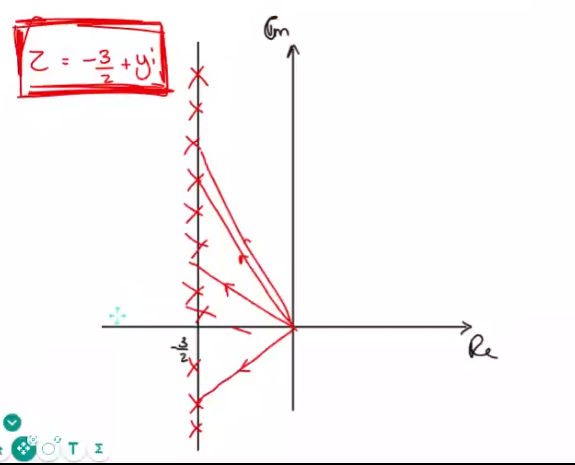
\includegraphics[scale=0.7]{ex1a complex loci}
		\end{center}
	\end{multicols}
	
	\begin{example}
		Given $\abs{\frac{z-1}{z+4i}} = 2 $ , find the locus of $z$.
	\end{example}
	Remembering: $\abs{\frac{z_1}{z_2}} = \frac{\abs{z_1}}{\abs{z_2}}$
	
	
	Let $z = x+yi$
	\begin{alignat*}{2}
		&                & \abs{\frac{z-1}{z+4i}} & = 2                   \\
		& \implies \quad & \abs{z-1}              & = 2\abs{z+4i}         \\
		& \implies \quad & \abs{(x-1)+yi}         & = 2\abs{x+(y+4)i}     \\
		& \implies \quad & \sqrt{(x-1)^2+y^2}     & = 2\sqrt{x^2+(y+4)^2} \\
		& \implies \quad & \sqrt{(x-1)^2+y^2}     & = 2\sqrt{x^2+(y+4)^2} \\
	\end{alignat*}
	\hrulefill
	\begin{example}
		Given that $z_A = \frac{1}{10} (-1+i)$ and $z_B = -\frac{1}{500} (11+127i)$ , find in the form a+bi the complex numbers $\frac{z_A}{z_B}$.
		If $P(x,y)$ is the point on the Argand diagram representing $z=x+yi$, determine the equation of the locus of $P$ where $\abs{z-z_A} = \abs{z-z_B}$.
	\end{example}
	$$\frac{z_A}{z_B}  =  \frac{1}{10} (-1+i) \div -\frac{1}{500} (11+127i)$$
	\begin{alignat*}{2}
		&   &                                     & =-5\cdot \frac{-1+i}{11+127i}                         \\
		&   &                                     & = \frac{5-5i}{11+127i} \cdot  \frac{11-127i}{11-127i} \\
		&   &                                     & = a+bi                                                \\
		&   & \therefore \quad a=-\frac{58}{1625} & ,\quad  b=-\frac{69}{1625}                            \\
		&   & \abs{z-z_A}                         & = \abs{z-z_B}                                         
	\end{alignat*}
	\newpage
	\begin{example}
		If the real part of $\dfrac{z+2}{z+2i}$ is equal to 1, show that the point $z$ lies on a straight line. Hence find the point $z_0$ on this line such that  $\abs{z_0} = \sqrt{2}$. Find also the quadratic equation with real coefficients which has $z_0$ as one of the roots.
	\end{example}
	
	Let $z = x+yi$\\
	\textbf{Showing that $\boldsymbol{z}$ lies on a straight line: }
	\begin{align*}
		&   & Re(\frac{z+2}{z+2i})           & = 1                                                                       \\
		&   & \implies \quad 1               & = Re(\frac{x+2+yi}{x+2i+yi})                                              \\
		&   & \implies \quad 1               & = Re\left(\frac{(x+2)+yi}{x+(y+1)i}\cdot \frac{x-(y+1)i}{x-(y+1)i}\right) \\
		&   & \implies \quad 1               & = Re\left(\frac{x(x+2) -i(y+2)(x+2) + iyx + y(2+y}{x^2 + (y+2)^2}\right)  \\
		&   & \implies \quad 1               & = \frac{x(x+2) + y(y+2)}{x^2 + (y+2)^2}                                   \\
		&   & \implies \quad x(x+2) + y(y+2) & = x^2  + y^2+4y+4                                                         \\
		&   & \implies \quad 2y              & = 2x-4                                                                    \\
	\end{align*}
	$$\therefore \quad y = x-2 \qed$$
	$$\text{Point } z \text{ lies on the straight line } y = x-2$$
	
	\begin{example}
		Shade on an Argand diagram the area represented by $\abs{z+i} < 4$.
	\end{example}~\\
	\setlength{\columnseprule}{0pt}
	\textbf{Finding the loci: }
	\begin{multicols}{2}
		\begin{center}
			\begin{align*}
				&   & \abs{z+i} & = \abs{x+(y+1)i}                                   \\
				&   &           & =\sqrt{x^2  + (y+1)^2}                             \\
				&   &           & =\sqrt{(x-0)^2 + (y-(-1))^2}                       \\
				&   &           & \text{ is the distance from point (0,-1) to (x,y)} 
			\end{align*}
		\end{center}
		\begin{center}
			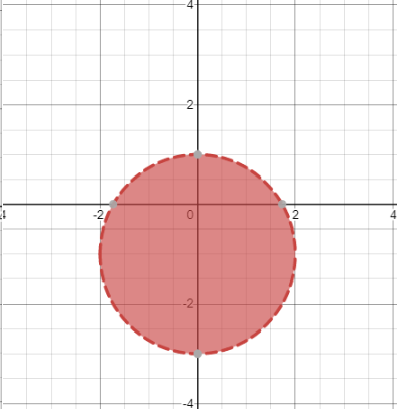
\includegraphics[scale=0.4]{complex_loci_ex5_circle}
		\end{center}
	\end{multicols}


	\textbf{Finding $\boldsymbol{z_0= (a,b) = a+bi\colon}$}
	\reqnomode
	
	\begin{alignat*}{2}
		&               & z_0           & = a+bi           \\
		& \implies      & \abs{z_0}     & = \sqrt{a^2+b^2} \\
		\intertext{Given:  $\abs{z_0}= \sqrt{2}$}
		& \implies\quad & \sqrt{a^+b^2} & = \sqrt{2}       \\
		& \implies\quad & a^2+b^2       & = 2\tag{1}       \\
		\intertext{We also know $z_0$ is on the line $y=x-2$}
		\therefore    b  = a-2\tag{2}	
		\intertext{Substituting 2 in 1: }
		&               & a^2 + (a-2)^2 & = 2              \\
		& \implies\quad & 2a^2 - 4a+4   & = 2              \\
		& \implies\quad & a^2-2a+1      & =0               \\
	\end{alignat*}
	$$	\therefore\quad z_0 = 1-i \qed$$\\
	\textbf{Finding quadratic equation with roots: $\boldsymbol{z_0, \bar{z_0}}$}
	\begin{center}
		$$x^2 - (\text{sum of roots})x + (\text{product of roots}) = 0$$
		$$\implies x^2 - (1-i + 1+i)x + (1-i)(1+i)=0$$
		$$\implies x^2-2x+2 = 0\qed$$
	\end{center}
	
\end{document}
	%	\begin{document}
	\chapter{Integration}
	\section{Reduction Formul\ae}
	Integrating using a reduction formula is in essence repeating integration by parts over and over again.\\
	
	
	 We can think of the process of finding a reduction formula for a given integral as a \emph{recursive approach} to integration by parts. By listing all the iterations of $\textstyle\int u\od vx\,dx= uv-\int v\od ux\,dx$, more specifically the $\textstyle\int v\od ux\,dx$ part in terms of $I_n$ where $n$ is the \emph{iterative index}, or the \textit{step number}, if you will.\\
	
	As expected, finding this recursively valid form is not as direct, and thus, the exponent has to be \textit{split} in such a way that trigonometric identities can be used.
	\begin{example}
		If $I_n = \int \cos^n x \, dx$ show that $I_n = \frac{1}{n} \sin\cos^{n-1}x + \frac{n-1}{n}\cdot I_{n-2}$. Hence find $\int \cos^5x\, dx$.
	\end{example}
	
	\begin{align*}
		I_n                  & = \int \cos^n x \, dx                                                       \\
		& = \int \cos x \cdot \cos^{n-1}x\, dx                                        \\
		%&\quad \text{Integrating by parts: }\\								
		\therefore \quad I_n & = \cos^{n-1}x\sin x + (n-1)\int\cos^{n-2}x\sin^2x\,dx                       \\
		& = \cos^{n-1}x\sin x + (n-1)\int\cos^{n-2}x(1-\cos^2x)\,dx                   \\
		& = \cos^{n-1}x\sin x + (n-1)\int\cos^{n-2}x \, dx \,-\, (n-1)\int\cos^nx\,dx \\
		& = \cos^{n-1}x\sin x + (n-1)I_{n-2} - (n-1)I_n                               \\
		I_n + (n-1)I_n       & = \cos^{n-1}x\sin x + (n-1)I_{n-2}                                          \\
		\implies  nI_n       & = \cos^{n-1}x\sin x + (n-1)I_{n-2}                                          \\
		\implies I_n         & = \frac1n\cos^{n-1}x\sin x + \left(\frac{n-1}n\right)I_{n-2}                \\
	\end{align*}
	
	\begin{align*}
		\int \cos^5 x \, dx   =\,      & I_5                                                                                                                 \\
		& I_5 = \frac{1}{5} \cos^4x\sin x + \frac45I_3                                                                        \\
		& I_3 = \frac{1}{5} \cos^4x\sin x + \frac{4}{5}I_1                                                                    \\
		& I_1 = \int \cos x \, dx = \sin x + k                                                                                \\
		\therefore \quad \int \cos^5 x & = \frac{1}{5}\cos^4x \sin x + \frac{4}{5}\left(\frac{1}{3}\cos^2x\sin x + \frac{2}{3}\left(\sin x + k\right)\right) \\
		& =\frac{1}{5}\cos^2x\cdot\sin x + \frac4{15} \cos^2 x \cdot \sin x + \frac{8}{15}\sin x + c   \qed                   
	\end{align*}	  						
		\hrulefill
	\begin{example}
		If $I_n = \int \tan^n\theta \, d\theta$, find a reduction formula for $I_n$ and use it to evaluate $\int_0^{\frac\pi4} \tan^6\theta\,d\theta$.
	\end{example}
	
	\begin{equation*}
		\begin{split}
			I_n &= \int \tan^n\theta \, d\theta\\
			&= \int \tan^2\theta \tan^{n-2}\theta\, d\theta\\
			&= \int (\sec^2\theta - 1) \tan^{n-2}\theta\, d\theta\\
			&= \int \sec^2\theta\tan^{n-2}\theta\,d\theta - \int \underbrace{\tan^{n-2}\theta\,d\theta}\\
			&= \frac{\tan^{n-1}\theta}{n-1} - \underbrace{I_{n-2}}
		\end{split}
		\qquad\qquad\qquad
		\begin{split}
			\int_0^{\frac\pi4}\tan^6\theta\,d\theta &= I_6\bigg|_0^{\frac\pi4}\\
			I_6 &= \frac{tan^5\theta}{5} - I_4\\
			I_4 &= \frac{\tan^3\theta}{3} - I_2\\		
			I_2 &= \tan\theta - I_0\\
			I_0 &= \int 1 \, d\theta = \theta + k
		\end{split}
	\end{equation*}
	\begin{align*}
		\therefore \int_0^\frac\pi4  \tan^6\theta \, d\theta & =  \frac{\tan^6\theta}5 - \frac{\tan^3\theta}{3} + \tan\theta - \theta\bigg|_0^\frac\pi4 \\
		& = \frac15 - \frac13 + 1 - \frac{\pi}{4}                                                  \\
		& = \frac{13}{15} - \frac{\pi}{4}   \qed                                                   
	\end{align*}
		\hrulefill\newpage
	
	\begin{example}
		Establish a reduction formula that could be used to find $\int x^ne^x \, dx$ and use it to find $\int x^4e^4$.
	\end{example}
	
	\begin{equation*}
		\begin{split}
			\text{Let } I_n &= \int x^ne^x \, dx \\
			\text{Let } u 	&= x^n    \qquad   \od{v}{x} = e^x \\
			\od{u}{x}     	&= nx^{n-1} \qquad  v = e^x         \\
			\therefore \quad I_n	&= x^ne^x - n \int x^{n-1}e^x \, dx\qquad\\
			&= x^ne^x - n\, I_{n-1}
		\end{split}
		\begin{split}
			&\int x^4e^x = I_4\\
			&I_4 = x^4e^x - 4I_3\\
			&I_3 = x^3e^x - 3I_2\\
			&I_2 = x^2e^x - 2I_1\\		
			&I_1 = xe^x - I_0\\				 		 	
			&I_0 = e^x + k
		\end{split}
	\end{equation*}
	\begin{align*}
		\therefore \quad I_4 & = x^4e^x -4(x^3e^x - 3(x^2e^x - 2(xe^x - e^x + k))) \\
		& = x^4e^x -4x^3e^x + 12x^2e^x - 24xe^x + 24e^x + c   \qed
	\end{align*}
		\hrulefill
	\begin{example}
		Establish a reduction formula which can be used to evaluate $\int x^n \sin x \, dx$.
	\end{example}
	
	\begin{align*}
		\text{Let } I_n &= \int x^n \cdot \sin x\\
						&= -x^n\cos x + \int nx^{n-1}\cos x\,dx\\
						&= -x^n\cos x + n\left(x^{n-1}\sin x - \int (n-1)x^{n-2}\sin x\,dx\right)\\
						&= -x^n\cos x + n\left(x^{n-1}\sin x - (n-1) \int x^{-2} \cdot x^n\sin x\,dx\right)\\
						&= -x^n\cos x + n\left(x^{n-1}\sin x - (n-1) \underbrace{x^{n-2}\sin x\,dx}\right)\\
						\therefore \quad I_n &= -x^n\cos x + n\left(x^{n-1}\sin x - (n-1)I_{n-2}\right)\\
						&= -x^n\cos x + nx^{n-1}\sin x - n(n-1)I_{n-2} \qed
	\end{align*}
	\hrulefill\newpage
	
	\begin{example}
		Establish a reduction formula to find $\int \csc^nx \, dx$. Hence find $\int csc^5x \, dx$
	\end{example}


	\begin{align*}
		\text{Let } I_n &= \int \csc^nx \, dx\\
		&= \int \csc^2x \cdot \csc^{n-2}x \, dx\\
		\text{Let } u & = \csc^{x-2} x              \qquad \od{v}{x} = \csc^2x \, dx \\
		\od{u}{x}     & = -(n-2)\csc^{n-2}\cot x  v \qquad = -\cot x                 \\
		\therefore \int \csc^nx \, dx &= -\cot x \cdot \csc^{n-2}x  - (n-2)\int \csc^{n-2}x\cot^2x \, dx\\
		I_n &= 	-\cot x \cdot \csc^{n-2}x - (n-2)\int \csc^{n-2}x\left(\csc^2x - 1\right) \, dx\\
		&= 		-\cot x \cdot \csc^{n-2}x - (n-2)\int \csc^{n}x\,dx + (n-2)\int\csc^{n-2}xdx\\
		&=-\cot x \cdot \csc^{n-2}x  - (n-2)\, I_n + (n-2)I_{n-2}\\
		I_n + nI_n -2I_n &= -\cot x\cdot \csc^{n-2}x  + (n-2)I_{n-2}\\
		(n-1)I_n &= -\cot x\cdot \csc^{n-2}x  + (n-2)I_{n-2}\\
		I_n &= \frac{-1}{n-1}-\cot x\cdot \csc^{n-2}x + \frac{n-2}{n-1}I_{n-2}\\
		&= \left(1-\frac{1}{n-1}\right)I_{n-2}-\frac{\cot x\csc^{n-2}x}{n-1}\qed
	\end{align*}
	\begin{example}
		Show that if $I_n - \int_0^\pi x^n\sin x\,dx$, then $I_n = \pi^n - n(n-1)\,I_n-1$. Hence evaluate $\int_0^\pi\sin x\,dx$
	\end{example}
	\begin{align*}
		I_n &=\left[-x^n\cos x\right]_0^\pi + n\int_0^\pi x^{n-1} \cos x \, dx\\
		&=\pi^n + n\int_0^\pi x^{n-1} \cos x \, dx\\
		&= \pi^n \int_0^\pi \\
		\text {Let } u &=
	\end{align*}
	\begin{example}
		Show that, if $I_n = \int_0^1 x^n e^{x^3} \, dx$, then $I_n =\frac{e}{3} - \frac{n-2}{3} \cdot I_{n-3}$
	\end{example}
	
	\begin{align*}
		I_n &= \int_0^1 x^n e^{x^3} \, dx\\
		&= \int_0^1 x^{n-2}x^2e^{x^3} \, dx\\
		\therefore \quad I_n &= \left[\frac{x^{n-2}e^{x^3}}3\right]_0^1 - \frac{n-2}3 \int_0^1 x^{n-3}{e^{x^3}} \, dx\\
		&= \frac{e}3 - \frac{n-2}3 \cdot I_{n-3}
	\end{align*}
	
	\begin{example}
		Show that, if $I_n= \int_0^1 x^n(1+x^5)^4 \, dx$, then $I_n = \frac1{n+21} \left[32-(n-4)\cdot I_{n-5}\right]$
	\end{example}
	
	\begin{align*}
		I_n                 & = \int_0^1 x^n(1+x^5)^4 \, dx                                                                           \\
		& = x^{n-4}x^4(1+x^5)^4\,dx                                                                               \\
		& =\left[x^{n-4} \frac{(1+x^5)^5}{25}\right]_0^1 - \frac{n-4}{25} \int x^{n-5}(1+x^5)^5\,dx               \\
		& = \frac{32}{25}  -\frac{n-4}{25} \int_0^1x^n-5(1+x^5)(1+x^5)^4\,dx                                      \\
		& = \frac{32}{25} - \frac{n-5}{25}\int_0^1x^{n-5}(1+x^5)^4\, dx - \frac{n-4}{25}\int_0^1x^n(1+x^5)^4\, dx \\
		& = \frac{32}{25} - \left(\frac{n-4}{25}\right)I_{n-5} - \left(\frac{n-4}{25}\right)I_n                   \\
		25I_n               & = 32 - (n-4)I_{n-5} - \left(\frac{n-4}{25}\right)\,I_n                                                  \\
		25I_n + nI_n - 4I_n & = 32-(n-4)\,I_{n-5}\\
		(n+21)I_n &= 32-(n-4)I_{n-5}\\
		I_n &= \frac{1}{n+21}\left(32-(n-4)I_{n-5}\right)
	\end{align*}
	\hrulefill
	\newpage
	\begin{example}
		Given $I_n = \int_0^1 (1+x^2)^{-n}\,dx$, show that $2n\,I_{n+1} = 2^{-n} + (2n-1)\,I_n$
	\end{example}
	\begin{align*}
		I_n                   & = \int_0^1 (1+x^2)^{-n}\,dx                                             \\
		& = \int_0^1  (1+x^2)^{-n}\cdot 1 \,dx                                    \\
		\therefore \quad  I_n & = -2nx^2(1+x^2)^{-(n+1)}\bigg|_0^1 + 2n \int_0^1x^2(1+x^2)^{-n-1}\,dx   \\
						   	  & =2^{-n} + 2n\int_0^1(x^2+1-1)(1+x^2)^{-(n+1)}\,dx                       \\
						      & =2^{-n} + 2n \int_0^1(1+x^2)^{-2}\,dx - 2n\int_0^1 (1+x^2)^{-(n+1)}\,dx \\
							  & = 2^{-n} + 2n\,I_n - 2n\,I_{n+1}                                        \\
           	      2n\,I_{n+1} & = 2^{-n} + (2n-1)\,I_n                                                 
	\end{align*}
\end{document}
		%\documentclass{standalone}
\begin{document}
\chapter{Applications of Calculus}
\section{Integrals}
\subsection{Volume of Revolution}

If part	of a curve and the area underneath is rotated about a straight line, the solid formed is called a solid of revolution.\\

Consider the graph $y=f(x)$ and suppose we  rotate the part of the curve from $x=a$ to $x=b$ about the x-axis. If the shaded area of $f(x)$ is notated about the $x$-axis the following shape is formed:

\begin{multicols}{2}
	\begin{center}
		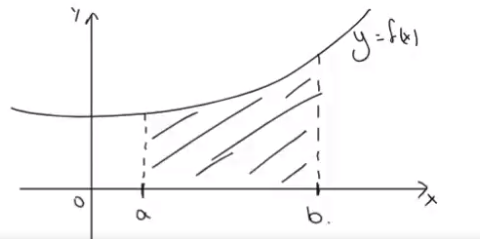
\includegraphics[scale=0.5]{app_of_calc_integ_1}
	\end{center}
	\begin{center}
		~\\
		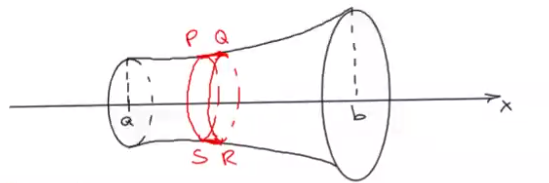
\includegraphics[scale=0.5]{app_of_calc_integ_2}
	\end{center}
\end{multicols}


Suppose that the solid formed is cut into sections as shown. Let $PQRS$ be a typical section. If the cuts are reasonably close to each other, $PQRS$ approximates a cylinder with height $\delta x$ and radius $y$ as shown below:
\begin{center}
	\qquad \qquad 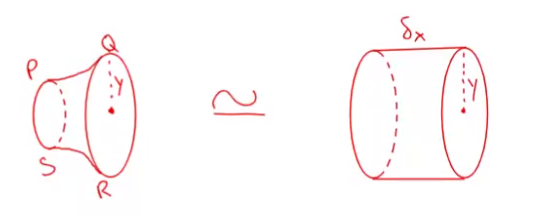
\includegraphics[scale=1]{app_of_calc_integ_3}
\end{center}
The volume, $\delta v$, of $PQRS$ is given by:
$$\delta V \simeq \pi y^2 \delta x$$
Thus, the volume $V$ of solid $PQRS$ is given by:
$$V\simeq \sum_{x=a}^{b} \pi y^2 \delta x$$
This summation approaches $V$ as $\delta x \to 0$
$$V = \lim\limits_{\delta x \to 0}   \sum_{x=a}^{b} \pi y^2 \delta x$$
$$\quad\boxed{V = \int_{a}^{b} \pi y^2 \, dx}$$
\hrulefill
\begin{example}
	Find the volume generated when the area  between $y=e^x$, the x-axis
\end{example}

\begin{alignat*}{2}
	&   & V & =\int_{0}^{1} \pi y \, dx \\
\end{alignat*}

\begin{example}
	Find the volume generated when the area defined by the inequalities $y\leq x^2$ and $y\geq x$ is rotated about the $x$-axis.
\end{example}
\begin{multicols}{2}
	\begin{tikzpicture}
		\begin{axis}[
			width=8cm,
			height=6cm,
			axis line style={-},
			xmin=0,
			xmax=2.5,
			ymin=0,
			ymax=2.5,
			xtick={}, % remove all ticks from x-axis
			ytick={}, % ditto for y-axis
			xlabel=$x$, 
			ylabel=$y$,
			axis lines=center, % default is to make a box around the axis
			samples=100]
			\addplot [name path=A,samples=501, domain=0:2, black] {sqrt(x)};
			\addplot [name path=B,samples=501, domain=0:2, green]  {x};
			\draw[pattern=north east lines,
			intersection segments={
				of=A and B,
				sequence={L2--R2[reverse]}
			}];
		\end{axis}
	\end{tikzpicture}
	\begin{center}
		
	\end{center}
	
\end{multicols}
\begin{alignat*}{2}
	&   & V_{e-c} & = V_e - V_c                                                      \\
	&   &         & = \pi \int_{0}^{1} \sqrt{x}^2 \, dx - \pi \int_{0}^{1} x^2 \, dx \\
\end{alignat*}
\begin{example}
	Find the volume generated when the area in the first quadrant bounded by the circle $x=4\cos\theta, y=4\sin\theta$ rotates completely about the $x$-axis.
\end{example}
\begin{example}
	
	Find the volume when the region defined by  $y\geq x^2+1,\quad x\geq0$ and $y\leq2$ is rotated about the $y$-axis.
\end{example}
\begin{tikzpicture}
	\begin{axis}[
		width=8cm,
		height=6cm,
		axis line style={-},
		xmin=0,
		xmax=2.5,
		ymin=0,
		ymax=2.5,
		xtick={}, % remove all ticks from x-axis
		ytick={}, % ditto for y-axis
		xlabel=$x$, 
		ylabel=$y$,
		axis lines=center, % default is to make a box around the axis
		samples=100]
		\path[name path=axis] (axis cs:0,0) -- (axis cs:0,2);
		\addplot [name path=A, domain=0:2, black] {2};	
		\addplot [name path=B, domain=0:2, black]  {x^2 + 1};
		\draw[pattern=north east lines,
		%TODO fix this
		intersection segments={
			of=B and A,
			of=axis and B,
			of=A and axis,
			sequence={L2--R	2[reverse]}
		}];
		%	\draw[pattern=north east lines,
		%	intersection segments={
		%		of=axis and B,
		%	}];
	\end{axis}
\end{tikzpicture}
\subsection{Length of an arc of a curve}
To find the length of an arc of a curve we use the method of summing small elements of one length.\\
Suppose that arc $PQ$, of length $\delta s$, is such an element. Then, the length $S$ of the curve $AB$ is given by:
\begin{multicols}{2}
	\begin{center}
		$\sum_{x=x_1}^{x_2} \delta S$
	\end{center}
	\begin{center}
		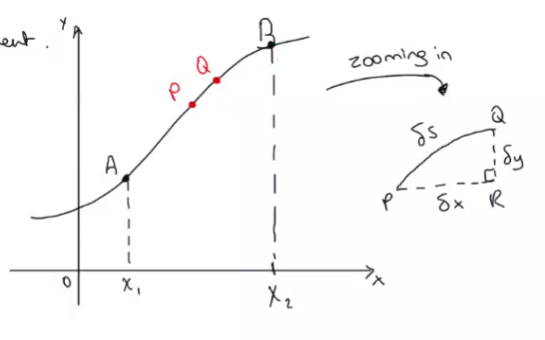
\includegraphics[width=0.7\linewidth]{app_of_integ_4}
	\end{center}
\end{multicols}


As $\delta s$ is very small, it can be approximated to the hypothenuse of the $\triangle PQR$. Thus:
\begin{alignat*}{2}
	&            & (\delta x)^2 + (\delta y)^2                    & \simeq (\delta s)^2                                                                 \\
	& \implies   & 1 + \left( \frac{\delta y}{\delta x}\right) ^2 & \simeq \left( \frac{\delta S}{\delta x}\right) ^2                                   \\
	& \implies   & \delta S                                       & \simeq \sqrt{1+\left( \frac{\delta y}{\delta x}\right)^2 } \delta x                 \\
	& \therefore & S                                              & \simeq \sum_{x=x_1}^{x_2} \sqrt{1 + \left(\frac{\delta y}{\delta x}\right)}\delta x 
\end{alignat*}
~\\
~\\
As $\delta x \leftarrow 0, (\frac{\delta y}{\delta x}) \leftarrow \frac{dy}{dx} \quad $and$ \quad s = \lim_{\delta x \to 0} \sum_{x=x_1}^{x_2} \sqrt{1+\left( \frac{\delta y}{\delta x}\right)^2}  \delta x$
~\\
~\\
~\\

\begin{center}
	\begin{tcolorbox}[center title,hbox,    
		lifted shadow={1mm}{-2mm}{3mm}{0.1mm}%
		{black!50!white}]
		\begin{varwidth}{\textwidth}
			\begin{center}
				$\therefore \quad S = \int_{x_1}^{x_2} \sqrt{1 + \left(\frac{dy}{dx}\right)^2}\, dx$
			\end{center}
		\end{varwidth}
	\end{tcolorbox} 
\end{center}


Knowing the Cartesian equation of the curve, the necessary integration can be carried out.\\

Let us now consider a curve $S$ parametrically in terms of $t$.

We can use again :
\begin{alignat*}{2}
	&          & (\delta s )^2                            & \simeq (\delta x)^2 + (\delta y)^2                                                                         \\
	& \implies & \left(\frac{\delta s}{\delta t}\right)^2 & \simeq \left(\frac{\delta x}{\delta t}\right)^2 + \left(\frac{\delta y}{\delta t}\right)^2                 \\
	& \implies & \delta s                                 & \simeq \sqrt{\left(\frac{\delta x}{\delta t}\right)^2 + \left(\frac{\delta y}{\delta t}\right)^2} \delta t 
\end{alignat*}

~\\
as $\delta t \to 0\quad ; \quad \frac{\delta x}{\delta t} \to \frac{dx}{dt} \quad \text{and} \quad \left(\frac{\delta y}{\delta t}\right) \to \frac{dy}{dt}$\\
~\\

$$\therefore S = \lim_{\delta t \to 0} \sum_{t=t_1}^{t_2} \sqrt{\left(\frac{\delta x}{\delta t}\right)^2 + \left(\frac{\delta y}{\delta t}\right)^2} \delta t$$

\begin{center}
	\begin{tcolorbox}[center title,hbox,    %%<<---- here
		lifted shadow={1mm}{-2mm}{3mm}{0.1mm}%
		{black!50!white}]
		\begin{varwidth}{\textwidth}
			\begin{center}
				$S = \int_{t_1}^{t_2} \sqrt{\left(\frac{dx}{dt}\right)^2 + \left(\frac{dy}{dt}\right)^2}\, dt$
			\end{center}
		\end{varwidth}
	\end{tcolorbox} 
\end{center}
\section{Rates of change}
The notation $\dfrac{dy}{dx}$ denotes the rate of change of $y$ w.r.t.x. Suppose that $x$ and $y$ are quantities a such as length and volume respectively. Then $\dfrac{dy}{dx}$ denotes the rate of change of volume w.r.t some length. In this section we use differentiation to deal with practical problems involving rates of change. 

\begin{example}
	A spherical balloon is blown up so that its volume increases at a constant rate of $2\text{cm}^3/s$. Find the rate of increase of the radius when the volume of the balloon is $50\text{cm}^3$
\end{example}

\begin{multicols}{2}
	$\od{V}{t} = 2$
	
\end{multicols}
\begin{example}
	A container with water is in the form of an inverted hollow cone with a iaerrentical angle of $30\degree$. Water drips out from the vertex at the rate $3\text{cm}^2/s$. Find the rate at which the surface area in contact with the water is changing when there are $8\pi\text{cm}^3$ of water remaining in the cone.
	
	\begin{figure}
		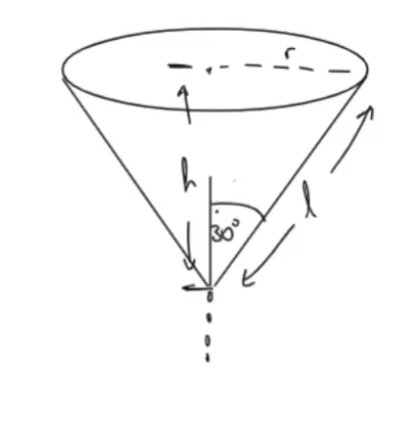
\includegraphics[scale=0.5]{app_of_calc_der_1}
	\end{figure}
	\begin{multicols}{2}
		\begin{align*}
			\od{V}{t} & = -3                            \\
			V         & = \frac{1}{3} \pi r^2 h         \\
			V         & = \frac{1}{3} \pi r^2 \sqrt{3}r \\
			V         & = \frac{\sqrt{3}}{3}\pi r^3     \\
			\od{V}{t} & = \sqrt{3}\pi  r^2              
		\end{align*}
		\begin{align*}
			\text{Required derivative: } \od{A}{t} &          \\
			A                                      & = \pi rl 
		\end{align*}
		
	\end{multicols}
\end{example}
\end{document}
	
%		%!TEX root = maths.tex
\usetikzlibrary{patterns,intersections,arrows,backgrounds}

\newcommand{\degre}{\ensuremath{^\circ}}
\pgfplotsset{compat=1.15}
\usetikzlibrary{arrows}


\newcommand{\realPlot}[2]{
	\draw[domain=#1,scale=1,samples=500 ] plot (\x:{#2}); %Curve with parameter
}


\newenvironment{fullPlot}[4]
{\begin{center}
		\resizebox{0.5\textwidth}{!}{%	
			\begin{tikzpicture}
			\begin{axis}[
			x=1cm,y=1cm,
			axis lines=middle,
			ymajorgrids=true,
			xmajorgrids=true,
			xmin=#1,
			xmax=#2,
			ymin=#3,
			ymax=#4,
			xtick={-20,-19,...,20},
			ytick={-20,-19,...,20},]
			\coordinate (origin) at (0,0);
			\end{axis}  
			\begin{scope}[shift={(origin)}]
			\clip (#1,#3) rectangle (#2,#4);
				%Dashed lines loop (increments of 15 degrees)
			\foreach \i in {0,15,...,75,105,120,...,180}{
				\draw[red,dashed, thick, samples=500] plot(\x, {tan(\i) * \x});}
				\draw[red, dashed, thick, samples=500] plot(0,\x);		 %Line x=0 due to tan() math err
		}
	
	
		{ 			
			%Green crosses loop (incremenets of 15 degress with upper bound parameter)
%			\foreach \x in {0,15,...,75,105,120,...,{#6}}{
%				\pic[line width=1pt,green] at ({\x}:{#5}) {mycross};}
			
			%	\pic[line width=1pt,green] at (0,5) {mycross};
			%	\pic[line width=1pt,green] at (0,-5) {mycross};
			\end{scope}
			\end{tikzpicture}
		}
	\end{center}

}	



\graphicspath{pictures/Polar_Curves}
\begin{document}
	\chapter{Polar Curves}
	\section{Introduction}
	The position of a point on a plane can be described in sever ways. With respect to some origin $O$
	we can locate a point $P$ on a plane by noting a horizontal distance followed by a vertical distance.\\
	
	\definecolor{uququq}{rgb}{0.25,0.25,0.25}
	\definecolor{xdxdff}{rgb}{0.49,0.49,1}
	\definecolor{qqqqff}{rgb}{0,0,1}
	\definecolor{xdxdff}{rgb}{0.49,0.49,1}
	\definecolor{qqqqff}{rgb}{0,0,1}
	\begin{center}
		\definecolor{xdxdff}{rgb}{0.49,0.49,1}
		\definecolor{qqqqff}{rgb}{0,0,1}
		\begin{tikzpicture}[line cap=round,line join=round,>=triangle 45,x=1.0cm,y=1.0cm]
		\draw[->,color=black] (-1,0) -- (5,0);
		\foreach \x in {-1,1,2,3,4}
		\draw[shift={(\x,0)},color=black] (0pt,2pt) -- (0pt,-2pt) node[below] {\footnotesize $\x$};
		\draw[->,color=black] (0,-1) -- (0,4);
		\foreach \y in {-1,1,2,3}
		\draw[shift={(0,\y)},color=black] (2pt,0pt) -- (-2pt,0pt) node[left] {\footnotesize $\y$};
		\draw[color=black] (0pt,-10pt) node[right] {\footnotesize $0$};
		\clip(-1,-1) rectangle (5,4);
		\draw [dash pattern=on 1pt off 1pt] (0,3)-- (4,3);
		\draw [dash pattern=on 1pt off 1pt] (2.08,3) -- (2,2.9);
		\draw [dash pattern=on 1pt off 1pt] (2.08,3) -- (2,3.1);
		\draw [dash pattern=on 1pt off 1pt] (4,0)-- (4,3);
		\draw [dash pattern=on 1pt off 1pt] (4,1.58) -- (4.1,1.5);
		\draw [dash pattern=on 1pt off 1pt] (4,1.58) -- (3.9,1.5);
		\begin{scriptsize}
		\fill [color=red] (4,3) circle (1.5pt);
		\draw[color=black] (4.31,3.19) node {$P$ ($x$, $y$)};
		\fill [color=qqqqff] (4,0) circle (1.5pt);
		\draw[color=black] (4.2,0.2) node {$X$};
		\fill [color=qqqqff] (0,3) circle (1.5pt);
		\draw[color=black] (0.2,3.19) node {$Y$};
		\end{scriptsize}
		\end{tikzpicture}
	\end{center}
	
	However the point $P$ can be located on a plane with respect to the origin $O$, a horizontal line and the distance of $P$ from $O$.\\
	
	\definecolor{ttttff}{rgb}{0.2,0.2,1}
	\definecolor{qqqqff}{rgb}{0,0,1}
	\definecolor{cqcqcq}{rgb}{0.75,0.75,0.75}
	\definecolor{ttttff}{rgb}{0.2,0.2,1}
	\definecolor{qqqqff}{rgb}{0,0,1}
	\begin{center}
		
		\begin{tikzpicture}[line cap=round,line join=round,>=triangle 45,x=1.0cm,y=1.0cm]
		\draw[->,color=black] (-1,0) -- (6,0);
		\foreach \x in {-1,1,2,3,4,5}
		\draw[shift={(\x,0)},color=black] (0pt,2pt) -- (0pt,-2pt) node[below] {\footnotesize $\x$};
		\draw[->,color=black] (0,-1) -- (0,6);
		\foreach \y in {-1,1,2,3,4,5}
		\draw[shift={(0,\y)},color=black] (2pt,0pt) -- (-2pt,0pt) node[left] {\footnotesize $\y$};
		\draw[color=black] (0pt,-10pt) node[right] {\footnotesize $0$};
		\clip(-1,-1) rectangle (6,6);
		\draw [shift={(0,0)},color=ttttff,fill=ttttff,fill opacity=0.1] (0,0) -- (0:0.71) arc (0:45:0.71) -- cycle;
		\draw (0,0)-- (3,3);
		\begin{scriptsize}
		\fill [color=qqqqff] (0,0) circle (1.5pt);
		\draw[color=black] (-0.4,-0.3) node {Pole};
		\fill [color=red] (3,3) circle (1.5pt);
		\draw[color=black] (3.52,3.21) node {$P$ ($r$, $\theta$)};
		\draw[color=black] (1.71,1.44) node {$r$};
		\draw[color=black] (0.46,0.2) node {$\theta$};
		\end{scriptsize}
		\end{tikzpicture}
		
	\end{center}
	
	This is the polar coordinate system where we refer to the origin as the pole and the horizontal line as the initial line. The anti clockwise angle is usually measured in the principal range $-\pi < \theta \leq \pi$.
	\newpage
	\section{Relationship between Polar and Cartesian Coordinates}
	
	Consider the following diagram showing the point P on the plane, both in Cartesian and Polar coordinates
	
	The above relationship can be used to convert from one form to another.
	\begin{example}
		Find the polar coordinates of the curve given by $y=x^2+y^2=2x$
	\end{example}
	
	\begin{alignat*}{2}
	& \qquad \quad x^2+y^2  &   & = 2x  \\    
	& \implies 2r\cos\theta &   & = r^2 \\
	& \implies 2\cos\theta  &   & = r   
	\end{alignat*}
	
	
	\hrulefill
	\begin{example}
		Find the Cartesian equation corresponding to the curves \textbf{a)} $r=4(1+\cos\theta)$ and \textbf{b)} $3 = r\sin 2\theta$.
	\end{example}
	\begin{equation*}
	\begin{split}
	r &= 4(1+\cos\theta)
	\end{split}
	\qquad \qquad \qquad
	\begin{split}
	3 &= r\sin2\theta\\
	3 &= 2r\sin\theta\cos\theta\\	
	3  &= 2x\sin\frac yr
	\end{split}
	\end{equation*}
	$$i^2 + 1^2 = 0$$
	
	\newpage
	\section{Sketching Polar Curves}
	\begin{example}
		Sketch the polar curve of $2+2\cos\theta$.
	\end{example}
	Observing the following sketch, it is shown that a line of symmetry is present in the $x$-axis for the \emph{cosine} function family.
	\begin{center}
		\resizebox{300pt}{!}{%
			\begin{tabular}{c|c|c|c|c|c|c|c|c|c}
				
				$\displaystyle\theta$ & $0$ & $\frac\pi6$ & $\frac\pi4$ & $\frac\pi3$ & $\frac\pi2$ & $\frac{2\pi}3$ & $\frac{3\pi}4$ & $\frac{5\pi}6$ & $\pi$ \\ \hline
				$r$                   & 4   & 3.7         & 3.4         & 3           & 2           & 1              & 0.6            & 0.3            & 0     
			\end{tabular}
		}
	\end{center}
	\begin{center}
		\begin{tikzpicture}[scale=1.7]
		\draw[thick,->,>=latex] (-3,0)--(5,0) node[above] {$x$};
		\draw[thick,->,>=latex] (0,-3)--(0,4) node[left] {$y$};
		\draw[domain=0:540,scale=1,samples=1000] plot (\x:{2+(2*cos(\x))});
		\clip (-3,-3) rectangle (6,4);
		
		% Draw dotted lines and crosses
		\foreach \i in {0, {pi/6},{pi/4}, {pi/3}, {2* pi / 3}, {3 * pi / 4}, {5 *pi / 6}, {pi}}{
			\draw[red, dashed, samples=500] plot(\x, {tan( deg(\i)) * \x});
			\pic[line width=1pt,green] at ({deg(\i)}:{2+(2*cos(deg(\i)))}) {mycross};}																																		
		\end{tikzpicture}
	\end{center}
	\newpage
	\begin{example}
		Sketch the graph with polar equation $r=3-2\cos\theta$.
	\end{example}
	Similarly to the above example, a line of symmetry is present in the $x$-axis.
	\begin{center}
		\resizebox{300pt}{!}{%
			\begin{tabular}{c|c|c|c|c|c|c|c|c|c}
				$\displaystyle\theta$ & $0$ & $\frac\pi6$ & $\frac\pi4$ & $\frac\pi3$ & $\frac\pi2$ & $\frac{2\pi}3$ & $\frac{3\pi}4$ & $\frac{5\pi}6$ & $\pi$ \\ \hline
				$r$                   & 1   & 1.3         & 1.6         & 2           & 3           & 4              & 4.4            & 4.7            & 5     
			\end{tabular}
		}
	\end{center}
	
	
	
	\begin{center}
		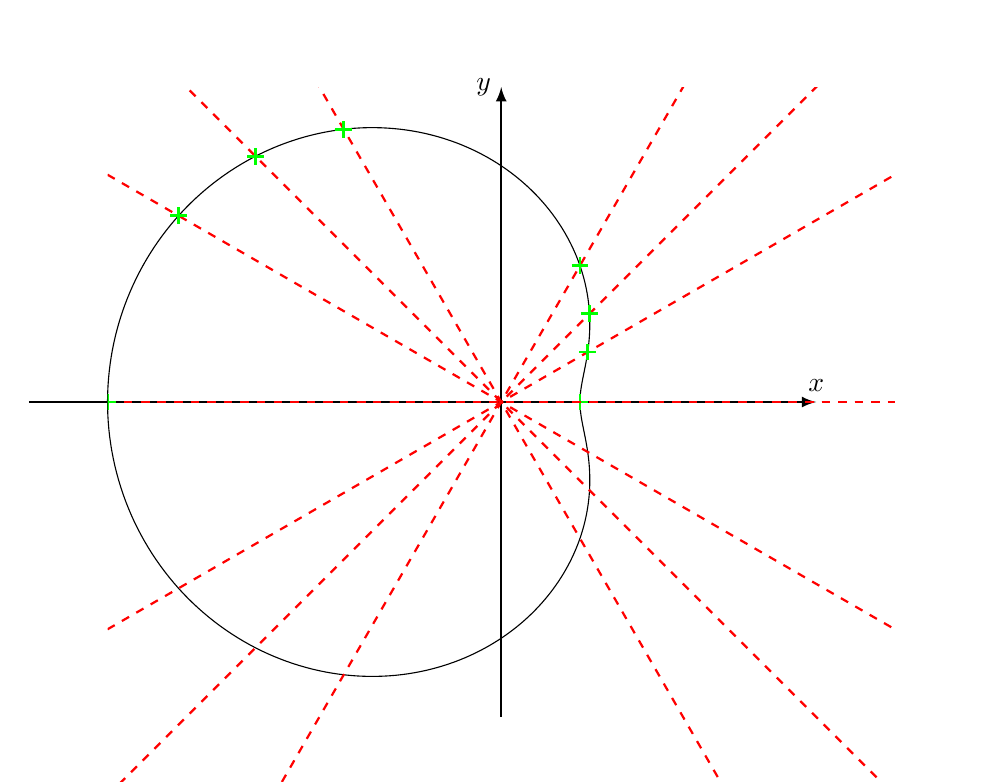
\begin{tikzpicture}
		\draw[thick,->,>=latex] (-6,0)--(4,0) node[above] {$x$};
		\draw[thick,->,>=latex] (0,-4)--(0,4) node[left] {$y$};
		\draw[domain=0:540,scale=1,samples=500] plot (\x:{3-(2*cos(\x))});
		\clip (-5,-5) rectangle (6,4);
		
		%	Draw dotted lines and crosses
		\foreach \i in {0, {pi/6},{pi/4}, {pi/3}, {2* pi / 3}, {3 * pi / 4}, {5 *pi / 6}, {pi}}{
			\draw[red, dashed, thick, samples=500] plot(\x, {tan( deg(\i)) * \x});
			\pic[line width=1pt,green] at ({deg(\i)}:{3-(2*cos(deg(\i)))}) {mycross};}
		\end{tikzpicture}
	\end{center}
	\newpage
	\begin{example}
		Sketch the graph with polar equation $r=5+2\sin\theta$.
	\end{example}
	
	It is noted that since the graph is part of the \emph{sine} function family,the line of symmetry is now present in the $y$-axis.
	
	\begin{center}
		\resizebox{300pt}{!}{%
			\begin{tabular}{c|c|c|c|c|c|c|c|c|c}
				$\theta$ & $\frac{-\pi}2$ & $\frac{-\pi}3$ & $\frac{-\pi}4$ & $\frac{-\pi}6$ & 0   & $\frac\pi6$ & $\frac\pi4$ & $\frac\pi3$ & $\frac\pi2$ \\ \hline
				$r$      & 3              & $3.3$          & $3.6$          & $4$            & $5$ & $6$         & $6.4$       & $6.7$       & $7$         
			\end{tabular}
		}
	\end{center}
	
	\begin{center}
		\begin{tikzpicture}
		\draw[thick,->,>=latex] (-8,0)--(6,0) node[above] {$x$};
		\draw[thick,->,>=latex] (0,-4)--(0,9) node[left] {$y$};
		\draw[domain=0:540,scale=1,samples=500] plot (\x:{5+(2*(sin(\x)))});
		
		\clip (-9,-4) rectangle (8,8);
		
		%	Draw dotted lines and crosses
		\foreach \i in {{-pi/6},{-pi/4}, {-pi/3}, 0, {pi/6},{pi/4}, {pi/3}}{
			\draw[red, dashed, thick, samples=500] plot(\x, {tan( deg(\i)) * \x});
			\pic[line width=1pt,green] at ({deg(\i)}:{5+(2*(sin(deg(\i))))}) {mycross};}
		\end{tikzpicture}
	\end{center}
	
	\newpage
	\begin{example}
		Sketch the polar curve $r=3+7\sin\theta$ and the circle $r=5$. Find the polar coordinates of their points of intersection.
	\end{example}
	
	\begin{center}
		\begin{tikzpicture}
		\draw[thick,->,>=latex] (-7,0)--(7,0) node[above] {$x$};
		\draw[thick,->,>=latex] (0,-6)--(0,11) node[left] {$y$};
		\draw[domain=0:540,scale=1,samples=1000] plot (\x:{3+(7*sin(\x))}); %Curve
		\draw[domain=0:540,scale=1,samples=500] plot (\x:5);				%Circle
		\clip (-7,-2) rectangle (6,10);
		
		%Draw dotted lines and crosses
		\foreach \i in {{-pi/6},{-pi/4}, {-pi/3}, 0, {pi/6},{pi/4}, {pi/3}}{
			\draw[red, dashed, thick, domain=-7:7, samples=500] plot(\x, {tan( deg(\i)) * \x});
			\pic[line width=1pt,green] at ({deg(\i)}:{3+(7*sin(deg(\i)))}) {mycross};}
		
		\draw[red, dashed, thick, domain=-7:12, samples=500] plot(0,\x);
		%Tangential Asymptotes
		\pic[line width=1pt,green] at ({deg(pi/2)}:10) {mycross};
		\pic[line width=1pt,green] at ({deg(-pi/2)}:-4) {mycross};
		
		\end{tikzpicture}
	\end{center}
	
	
	\newpage
	\begin{example}
		Sketch the polar curve $r=8\sin^2\theta$ and the line $r=\csc\theta$. Find the polar coordinates of their points of intersection.
	\end{example}
	\begin{center}
		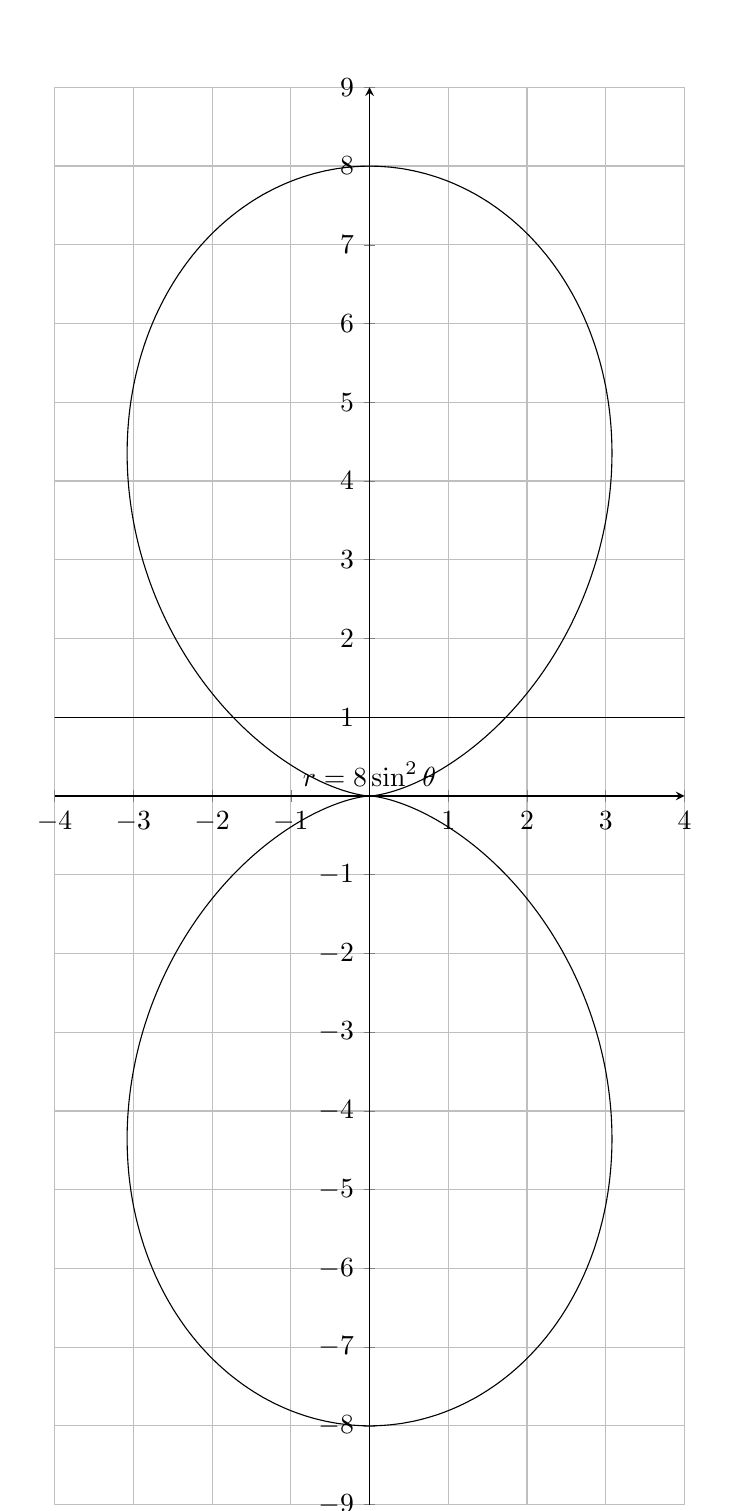
\begin{tikzpicture}
		\begin{axis}[
		x=1cm,y=1cm,
		axis lines=middle,
		ymajorgrids=true,
		xmajorgrids=true,
		xmin=-4,
		xmax=4,
		ymin=-9,
		ymax=9,
		xtick={-4,-3,...,4},
		ytick={-9,-8,...,9},]
		\draw[domain=0:540,scale=1,samples=1000] plot (\x:{8*(sin(\x)^2)}) node[above] {$r=8\sin^2\theta$}; %Curve
		\draw[domain=-5:5,scale=1,samples=1000] plot (\x, 1) node[above] {$r=\csc\theta$}; %Curve
		%	\clip (-7,-2) rectangle (6,10);
		\end{axis}
		\end{tikzpicture}
	\end{center}
	
	\section{Area partly bounded by a polar curve}
	Consider the following diagram showing the graph of $r=f(\theta)$.
	
	\begin{center}
		\resizebox{300pt}{!}{%
			\definecolor{ccffww}{rgb}{0.8,1,0.4}
			\definecolor{qqttcc}{rgb}{0,0.2,0.8}
			\definecolor{uuuuuu}{rgb}{0.26666666666666666,0.26666666666666666,0.26666666666666666}
			\definecolor{xdxdff}{rgb}{0.49019607843137253,0.49019607843137253,1}
			\begin{tikzpicture}[line cap=round,line join=round,>=triangle 45,x=1cm,y=1cm]
			\begin{axis}[
			x=1cm,y=1cm,
			axis lines=middle,
			ymajorgrids=true,
			xmajorgrids=true,
			xmin=-4.087350135407929,
			xmax=12.075704876608706,
			ymin=-1.9400069331551724,
			ymax=8.089791136292845,
			xtick={-4,-3,...,12},
			ytick={-1,0,...,8},]
			\clip(-4.087350135407929,-1.9400069331551724) rectangle (12.075704876608706,8.089791136292845);
			
			\fill[line width=0.8pt,color=ccffww,fill=ccffww,fill opacity=0.55] (1.6469997622170334,5.285200045490499) -- (1.8018963690587861,5.303857839349265) -- (2.057802642713001,5.344452622890168) -- (2.2425420008780867,5.375610046949744) -- (2.4085986469696503,5.401170598203379) -- (2.6317350137162325,5.427157717856224) -- (2.826543364850297,5.438046959825773) -- (2.9930508460166525,5.436092904437624) -- (3.1583701235903847,5.422111858769122) -- (3.394065928081652,5.378740328890088) -- (3.5780745473050493,5.323957494370168) -- (3.7684491850962933,5.246759511526517) -- (3.909043353636018,5.175946821869229) -- (4.096867913840399,5.062840104074621) -- (4.339673854011711,4.885528774754539) -- (4.70860996427174,4.552297629385634) -- (5.130951567039364,4.088855310480258) -- (5.420878217861827,3.7324711921147538) -- (5.752127039672099,3.3035617372125) -- (5.8996282307282275,3.1102010591021587) -- (0,0) -- cycle;
			\draw [line width=2pt,dash pattern=on 1pt off 1pt,domain=-4.087350135407929:12.075704876608706] plot(\x,{(-0--4.099788120747726*\x)/1.2775959286106953});
			\draw [line width=2pt,dash pattern=on 1pt off 1pt,domain=-4.087350135407929:12.075704876608706] plot(\x,{(-0--4.87618*\x)/9.24945});
			\draw[line width=2pt,color=xdxdff,smooth,samples=100,domain=-4.087350135407929:12.075704876608706] plot(\x,{0.014635180803888441*(\x)^(4)-0.23126329831793696*(\x)^(3)+1.0699408938350827*(\x)^(2)-1.8059409257011467*(\x)+6.282771603030379});
			\draw (2.6126764256158723,7.846889871240623) node[anchor=north west] {$\theta = \alpha$};
			\draw (7.440339068528793,5.195217727753861) node[anchor=north west] {$\theta = \beta$};
			\draw [line width=2.4pt,color=qqttcc,fill=qqttcc,fill opacity=0.1] (0,0) -- (27.797567846322046:0.9614841741650471) arc (27.797567846322046:72.69166717480417:0.9614841741650471) -- cycle;
			\draw [color=xdxdff](-2.5287336846561685,8.960187336063308) node[anchor=north west] {$ r=f({\theta})$};
			\begin{scriptsize}
			\draw [fill=uuuuuu] (1.6469997622170334,5.285200045490499) circle (2pt);
			%				\draw[color=uuuuuu] (1.74734066886733,5.524146524178746) node {$G$};
			\draw [fill=uuuuuu] (0,0) circle (2pt);
			\draw [fill=uuuuuu] (5.8996282307282275,3.1102010591021587) circle (2pt);
			\draw[color=uuuuuu] (6.038596351456593,3.3937000119498784) node {$D_1$};
			\draw[color=qqttcc] (1.0743017469517973,0.5143079324766583) node {$\omega$};
			\end{scriptsize}
			\end{axis}
			\end{tikzpicture}
		}
	\end{center}
	It can be shown that the area bounded by the curve $r=f(\theta)$, from $\theta = \alpha$ to $\theta = \beta$ is given by \[A = \frac12\int_\alpha^\beta r^2\,d\theta\]
	\hrulefill
	\newpage
	\begin{example}
		Sketch the curve with polar equation $r=2(1-\cos\theta)\sqrt{\sin\theta}$ for $0 \leq \theta\leq \pi$ and find the area it encloses.
	\end{example}
	\begin{center}
		\begin{tabular}{c|c|c|c|c|c|c|c|c|c|c|c|c|c}
			$\theta$ & 0   & $\frac{\pi}{12}$ & $\frac{\pi}6$ & $\frac{\pi}4$ & $\frac{\pi}3$ & $\frac{5\pi}{12}$ & $\frac\pi2$ & $\frac{7\pi}{12}$ & $\frac{2\pi}3$ & $\frac{3\pi}4$ & $\frac{5\pi}6$ & $\frac{11\pi}{12}$ & $\pi$ \\ \hline
			$r$      & $0$ & $0.03$           & $0.2$         & $0.5$         & $0.9$         & $1.5$             & $2$         & $2.5$             & $11$           & $2.9$          & $2.6$          & $2$                & $0$   
		\end{tabular}
	\end{center}
	
	\begin{fullPlot}{-3}{2}{-2}{3}
	\realPlot{0:180}{2*(1-cos(\x))*(sqrt(sin(\x)))}
	\end{fullPlot}
%	\fullPlot{-3}{2}{-2}{3}{2*(1-cos(\x))*(sqrt(sin(\x)))}{180}
	\begin{align*}
	A & =\frac12\int_0^\pi \left(2(1-\cos\theta)\sqrt{\sin\theta}\right)^2\,d\theta             \\
	& = \frac12\int_0^\pi 4(1-\cos\theta)^2\sin(\theta)\,d\theta                                \\
	& = 2\int_0^\pi \sin(\theta)(1-2\cos(\theta)+\cos^2\theta)\,d\theta\\
	&= 2\int_0^\pi \sin\theta - 2\sin\theta\cos\theta+\sin\theta\cos^2\theta\,d\theta\\
	&= 2\left(\left.-\cos\theta + \cos^2\theta - \frac{\cos^3\theta}{3}\right|_0^\pi\right)
	\end{align*}
	\newpage
	\begin{example}
		Sketch the curve with polar equation $r=3-4\cos\theta$ and find the area enclosed by the inner loop.
	\end{example}
	
	\fullPlot{-5}{5}{-5}{5}{2+2*(cos(\x))}{180}
	\newpage
	\begin{example}
		Sketch the curve  $r=5\sin3\theta$ and the circle $r=5$. Find the area of the region which lies inside the circle but outside the curve.
	\end{example}
	\begin{center}
		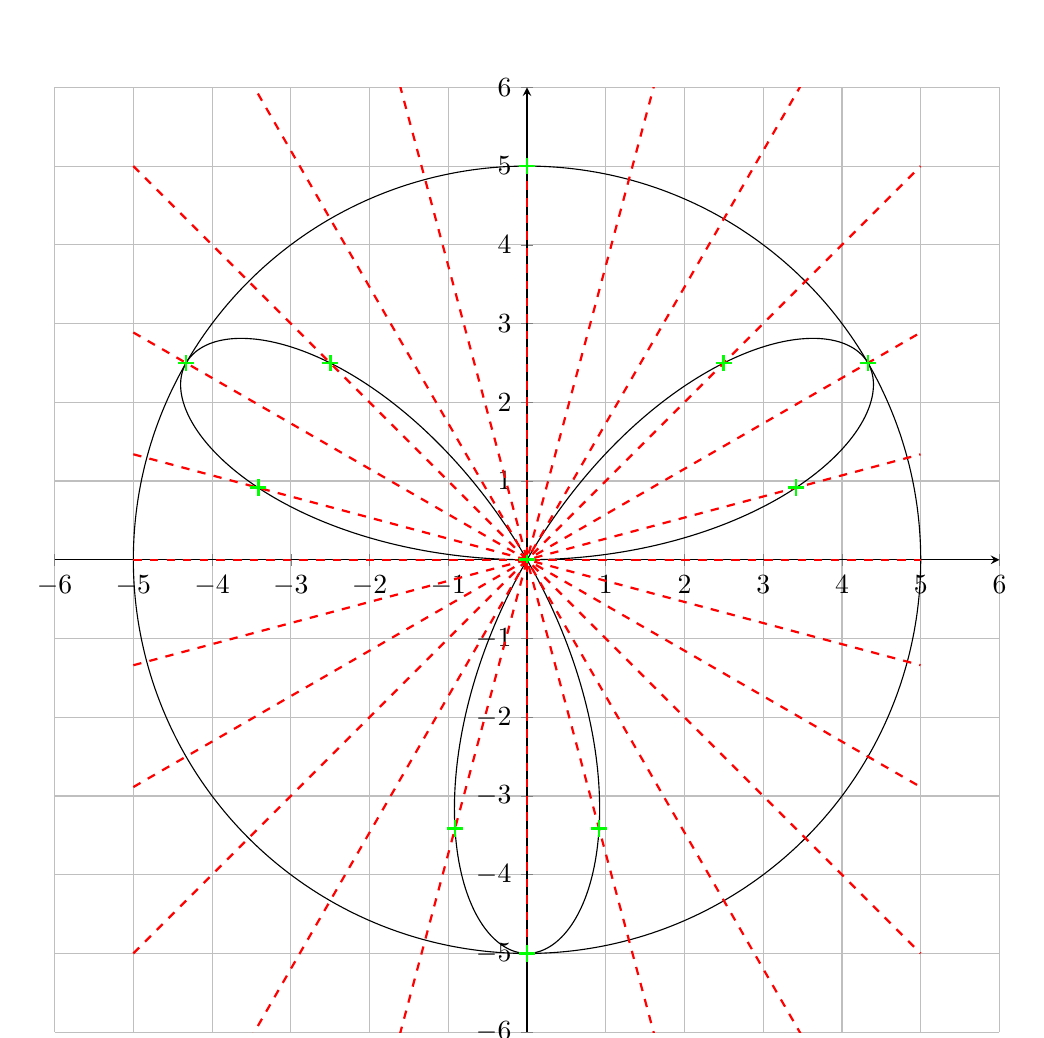
\begin{tikzpicture}
		\begin{axis}[
		x=1cm,y=1cm,
		axis lines=middle,
		ymajorgrids=true,
		xmajorgrids=true,
		xmin=-6,
		xmax=6,
		ymin=-6,
		scale=1,
		ymax=6,
		xtick={-6,-5,...,6},
		ytick={-6,-5,...,6},]
		\coordinate (origin) at (0,0);
		\end{axis}  
		\begin{scope}[shift={(origin)}]
		\clip (-6,-6) rectangle (6,6);
		\draw[domain=0:360,scale=1,samples=500 ] plot (\x:{5*sin(3*\x)}); %Curve 
		\draw[domain=0:360,scale=1,samples=500 ] plot (\x:5); %Curve 
		\foreach \i in {0,15,...,75,105,120,...,180}{
			\draw[red, dashed, thick, domain=-5:5, samples=500] plot(\x, {tan(\i) * \x});
			\pic[line width=1pt,green] at ({\i}:{5*sin(3*\i)}) {mycross};
		}
		\draw[red, dashed, thick, domain=-5:5, samples=500] plot(0, \x);
		\pic[line width=1pt,green] at (0,5) {mycross};
		\pic[line width=1pt,green] at (0,-5) {mycross};
		\end{scope}
		\end{tikzpicture}
	\end{center}
	
	
	\begin{multicols}{2}
		\noindent
		\begin{align*}
		A & = \frac12 \int_0^\frac\pi3 (5\sin(3\theta))^2\,d\theta                        \\
		& = \frac{25}{2} \int_0^\frac\pi3 \sin^2(3\theta)\,d\theta                      \\
		& = \frac{25}{2} \int_0^\frac\pi3 \frac{1-\cos(6\theta)}{2}                     \\
		& = \frac{25}{4} \left.\quad\theta - \frac{\cos(6\theta)}{6}\right|_0^\frac\pi3 \\
		& = \frac{25}{24} \left.\quad 6\theta - \cos6\theta\right|_\alpha^\beta          
		\end{align*}
		
		\begin{align*}
		A & = \pi r^2 \\
		& = 25\pi   \\~\\~\\~\\~\\
		\end{align*}
	\end{multicols}
	
	\newpage
	\begin{example}
		Sketch the curve $r=3(1+\sqrt{2}\cos\theta)$ and the line $r=3\sqrt{2}\sec\theta$. Find the polar coordinates of their points of intersection. Find the area of the region which lies inside the circle but outside of the cardioid.
	\end{example}
	
	
	\begin{center}
		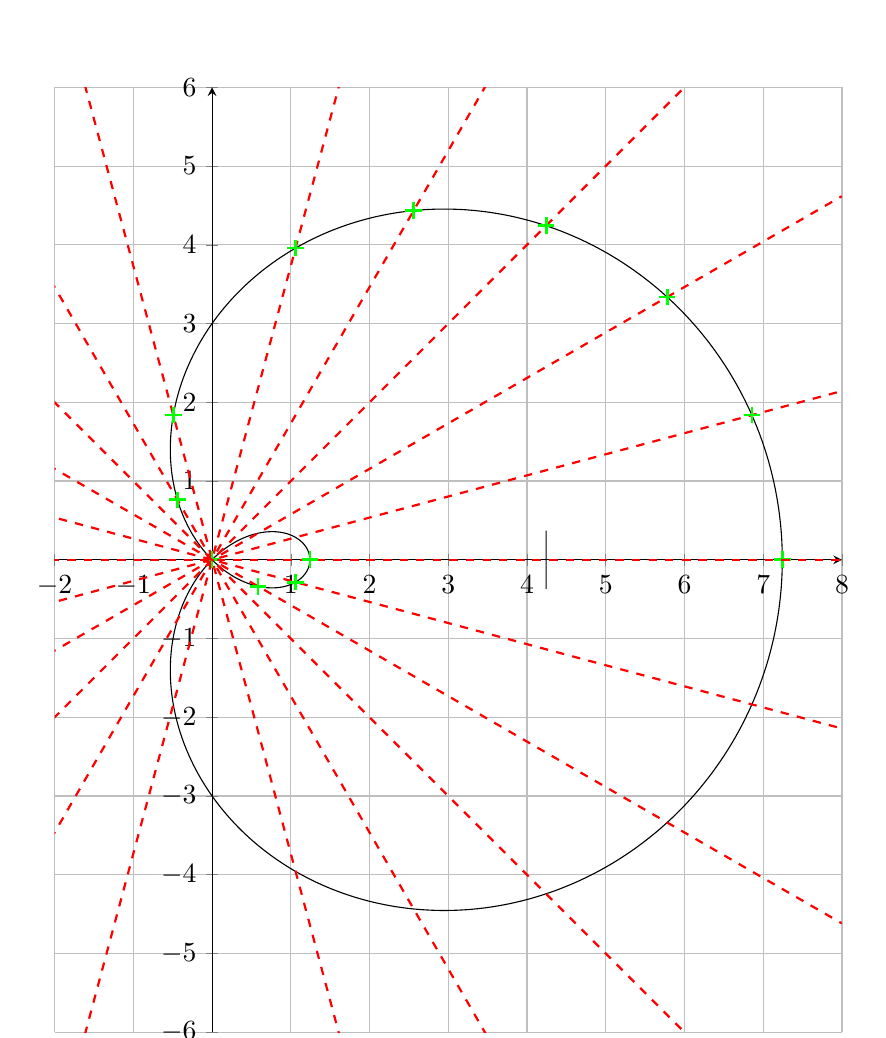
\begin{tikzpicture}
		\begin{axis}[
		x=1cm,y=1cm,
		axis lines=middle,
		ymajorgrids=true,
		xmajorgrids=true,
		xmin=-2,
		xmax=8,
		ymin=-6,
		scale=1,
		ymax=6,
		xtick={-2,-1,...,8},
		ytick={-6,-5,...,6},]
		\coordinate (origin) at (0,0);
		\end{axis}  
		\begin{scope}[shift={(origin)}]
		\clip (-2,-6) rectangle (8,6);
		\draw[domain=0:360,scale=1,samples=500 ] plot (\x:{3*(1+(sqrt(2)*cos(\x))}); %Curve 
		\draw[range=0:180,scale=1,samples=500 ] plot (\x:{3*sqrt(2)*sec(\x)}); %Curve 
		\foreach \i in {0,15,...,75,105,120,...,180}{
			\draw[red, dashed, thick, domain=-5:8, samples=500] plot(\x, {tan(\i) * \x});
			\pic[line width=1pt,green] at ({\i}:{3*(1+(sqrt(2)*cos(\i))}) {mycross};
		}
		%	\draw[red, dashed, thick, domain=-5:5, samples=500] plot(0, \x);
		%	\pic[line width=1pt,green] at (0,5) {mycross};
		%	\pic[line width=1pt,green] at (0,-5) {mycross};
		\end{scope}
		\end{tikzpicture}
	\end{center}
	\newpage
	
	\begin{example}
		Sketch the curve $r=5+\sin\theta$ and the line $r\sin\theta = 8$.
	\end{example}
	
	
	\begin{center}
		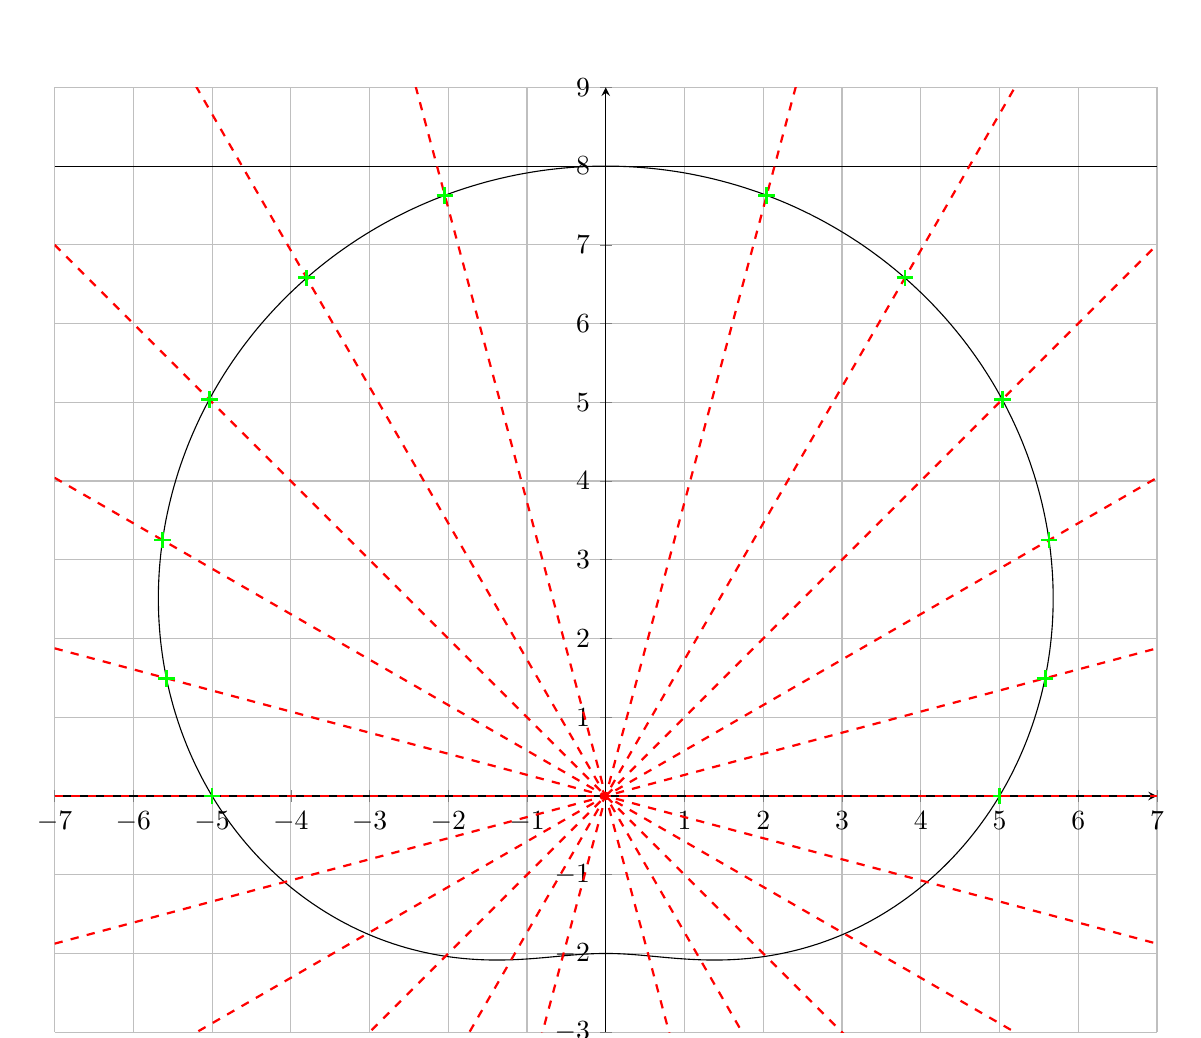
\begin{tikzpicture}
		\begin{axis}[
		x=1cm,y=1cm,
		axis lines=middle,
		ymajorgrids=true,
		xmajorgrids=true,
		xmin=-7,
		xmax=7,
		ymin=-3,
		scale=1,
		ymax=9,
		xtick={-7,-6,...,7},
		ytick={-3,-2,...,9},]
		\coordinate (origin) at (0,0);
		\end{axis}  
		\begin{scope}[
		shift={(origin)}]
		\clip (-7,-3) rectangle (7,9);
		\draw[domain=0:360,scale=1,samples=500 ] plot (\x:{5+(3*sin(\x))}); %Curve 
		\draw[domain=-7:7,scale=1,samples=500 ] plot (\x,8); %LIne y=8 
		\foreach \i in {0,15,...,75,105,120,...,180}{
			\draw[red, domain=-7:7,dashed, thick, samples=500] plot(\x, {tan(\i) * \x});
			\pic[line width=1pt,green] at ({\i}:{5+(3*sin(\i))}) {mycross};
		}
		%	\draw[red, dashed, thick, domain=-5:5, samples=500] plot(0, \x);
		%	\pic[line width=1pt,green] at (0,5) {mycross};
		%	\pic[line width=1pt,green] at (0,-5) {mycross};
		\end{scope}
		\end{tikzpicture}
	\end{center}
	
	
\end{document}
%		%!TEX root = maths.tex
\newcommand{\adj}{\text{adj}\,}
\newcommand{\identitymatrix}{\begin{bmatrix*}[c]1&0&0\\0&1&0\\0&0&1\end{bmatrix*}}
\begin{document}
\chapter{Matrices II}
\section{Determinant of a 3x3 Matrix}
The determinant of a 3x3 matrix is calculated by extracting a row of 2x2 determinants from the given 3x3 matrix. These 2x2 determinants are referred to as minors.

\begin{example}
	Find the determinant of the matrix $\mathbf A = \left(\begin{smallmatrix*}[r]
	2 &-1 &4\\
	3 &0 &-3\\
	4 &5 &6
	\end{smallmatrix*}\right)$
\end{example}
\section{[Parentheses about vector product]}
Consider the vectors $\mathbf{a} = x_1\mathbf{i} + y_1\mathbf{j} + z_1\mathbf{k}$ and b $\mathbf{b} = x_2\mathbf{i} + y_2\mathbf{j} + z_2\mathbf{k}$.\\

Since vector product is distributive across addition:\\

\begin{align*}
	\mathbf{a} \times \mathbf{b} & = \left(  x_1\mathbf{i} + y_1\mathbf{j} + z_1\mathbf{k} \right) \times \left( x_2\mathbf{i} + y_2\mathbf{j} + z_2\mathbf{k} \right)\\
	&+\cancel{x_1x_2(\mathbf i \times \mathbf i)} + x_1y_2(\mathbf i \times \mathbf j) + x_1z_2(\mathbf i \times \mathbf k)\\
	&+ y_1x_2(\mathbf j \times \mathbf i) + \cancel{y_1y_2(\mathbf j \times \mathbf j)} + y_1z_2(\mathbf j \times \mathbf k)\\
	&+z_1x_2(\mathbf k \times \mathbf i) + z_1y_2(\mathbf k \times \mathbf j) + \cancel{z_1z_2(\mathbf k \times \mathbf k)}\\
	&=x_1y_2\mathbf k - x_1z_2\mathbf j - y_1x_2 \mathbf k + y_1z_2\mathbf i +z_1x_2\mathbf j -z_1y_2\mathbf i\\
	&=(y_1z_2-z_1y_2)\mathbf i - (x_1z_2 - z_1 x_2)\mathbf j + (x_1y_2-y_1x_2)\mathbf k
\end{align*}

\section{Some properties of determinant}
The value of the determinant is unaltered if all the rows and columns of a given matrix are interchanged. If the above happens, the resulting determinant will be of opposite sign.\\
 If one row/column of a determinant $D$ is multiplied by $\lambda$, the resulting determinant is equal to $\lambda D$

\section{The Inverse of a 3x3 matrix}


\subsection{Matrix of cofactors}
Consider the matrix $\mathbf A = \begin{bmatrix}a&b&c\\d&e&f\\g&h&i\end{bmatrix}$\\

\noindent For each element of any given matrix $\mathbf A$:
	\begin{itemize}
\item{Ignore the values of the current row and column.}
\item{Calculate the determinant of the remaining values.}
\item{Apply alternating signs starting from $+$.}
\item{Input this determinant into a new matrix}
	\end{itemize}1
The result would be the below matrix referred to as \emph{the matrix of co-factors}.

\[
\mathbf C=
\begin{bmatrix*}[r]
	\begin{vmatrix}e&f\\h&i\end{vmatrix}&&-\begin{vmatrix}d&g\\f&i\end{vmatrix}&&\begin{vmatrix}d&e\\g&h\end{vmatrix}\phantom{-}\\\\
	-\begin{vmatrix}e&f\\h&i\end{vmatrix}&&\begin{vmatrix}d&g\\f&i\end{vmatrix}&&-\begin{vmatrix}d&e\\g&h\end{vmatrix}\phantom{-}\\\\
	\begin{vmatrix}e&f\\h&i\end{vmatrix}&&-\begin{vmatrix}d&g\\f&i\end{vmatrix}&&\begin{vmatrix}d&e\\g&h\end{vmatrix}\phantom{-}
\end{bmatrix*}
\]
\subsection{Adjugate matrix}
The next step of finding the inverse matrix of $\mathbf A$ is finding the \emph{adjugate} matrix of $\mathbf A$. This is done by obtaining the \emph{transpose} of the matrix of cofactors, in our case, $\mathbf C$.
\[
\adj A =
\begin{bmatrix*}[r]
\begin{vmatrix}e&f\\h&i\end{vmatrix}&&-\begin{vmatrix}e&f\\h&i\end{vmatrix}&&\begin{vmatrix}e&f\\h&i\end{vmatrix}\phantom{-}\\\\
-\begin{vmatrix}d&g\\f&i\end{vmatrix}&&\begin{vmatrix}d&g\\f&i\end{vmatrix}&&-\begin{vmatrix}d&g\\f&i\end{vmatrix}\phantom{-}\\\\
\begin{vmatrix}d&e\\g&h\end{vmatrix}&&-\begin{vmatrix}d&e\\g&h\end{vmatrix}&&\begin{vmatrix}d&e\\g&h\end{vmatrix}\phantom{-}
\end{bmatrix*}
\]
\subsection{Inverse matrix}
Let the inverse of a matrix $A$ be $A^{-1}$. It is defined as a matrix of the same size of $A$ such that \[AA^{-1} = A^{-1}A = I\]
This same matrix $A^{-1}$ is defined more particularly as \[A^{-1} = \frac{1}{\det A}\quad\text{adj }A\]
\begin{example}
	Find the inverse of the matrix $A = \begin{pmatrix*}
										2&3&1\\
										1&1&1\\
										5&-1&0
										\end{pmatrix*}$
	\end{example}
\begin{example}
Solve using the inverse matrix method the system of equations:\\
$x+y+z=7$\\
$x-y+2z=9$\\
$2x+y-z=1$
\end{example}
\newpage
\section{Transformation Matrices in 3D}
\subsection{Reflection along the xy plane}

\begin{center}
\begin{tikzpicture}[x=0.5cm,y=0.5cm,z=0.3cm,>=stealth]
% The axes
\draw[->] (xyz cs:x=-5) -- (xyz cs:x=5) node[above] {$x$};
\draw[->] (xyz cs:y=-5) -- (xyz cs:y=5) node[right] {$y$};
\draw[->] (xyz cs:z=-5) -- (xyz cs:z=5) node[above] {$z$};


\foreach \coo in {-4,-3,...,4}
{
	\draw (\coo,-1.5pt) -- (\coo,1.5pt);
	\draw (-1.5pt,\coo) -- (1.5pt,\coo);
	\draw (xyz cs:y=-0.15pt,z=\coo) -- (xyz cs:y=0.15pt,z=\coo);
}
%\draw (xyz cs:y=3,z=2);
\end{tikzpicture}
\end{center}


\begin{align*}
\begin{bmatrix*}[c]1&0&0\\0&1&0\\0&0&1\end{bmatrix*} \rightarrow \begin{bmatrix*}[c]1&0&0\\0&1&0\\0&0&-1\end{bmatrix*}
\end{align*}

\subsection{Rotation along the y-axis}

\begin{align*}
\begin{bmatrix*}[c]1&0&0\\0&1&0\\0&0&1\end{bmatrix*} \rightarrow \begin{bmatrix*}[c]\cos\theta&0&-\sin\theta\\0&1&0\\\sin\theta&0&\cos\theta\end{bmatrix*}
\end{align*}
\subsection{Rotation along the z-axis}

\begin{align*}
\begin{bmatrix*}[c]1&0&0\\0&1&0\\0&0&1\end{bmatrix*} \rightarrow \begin{bmatrix*}[c]\cos\theta&-\sin\theta&0\\\sin\theta&\cos\theta&0\\0&0&1\end{bmatrix*}
\end{align*}
\subsection{Rotation along the z-axis}

\begin{align*}
\begin{bmatrix*}[c]1&0&0\\0&1&0\\0&0&1\end{bmatrix*} \rightarrow \begin{bmatrix*}[c]1&0&0\\0&\cos\theta&-\sin\theta\\0&\sin\theta&\cos\theta\end{bmatrix*}
\end{align*}
\subsection{Enlargement}
When we enlarge (or conversely, reduce) by scale factor $n$, the unit base vector is multiplied by $n$.\\
Thus the matrix representing an enlargement by scale factor n is given by:
\begin{align*}
n\identitymatrix = \begin{bmatrix*}[c]n&0&0\\0&n&0\\0&0&n\end{bmatrix*}
\end{align*}
\section{Geometric Interpretation of the Determinant}
Consider an object with volume $V$ transformed by the matrix $\mathbf A$ with determinant $|\mathbf A|$. 
The volume of the image is given by $|\mathbf A|V$. Thus, the determinant of the transformation matrix denotes the number of times by which th volume of the object increases or decreases.
\begin{example}
	Describe the effect on volume in $3$D space of the transformation given by $\mathbf{A} = \begin{bmatrix*}[r]1&2&3\\5&0&-1\\2&4&-3\end{bmatrix*}$
\end{example}

\begin{example}
	Find the images of $P(4,5,1)$, $Q(3,-1,-2)$, $R(6,-2,0)$ under the transformation given by \\$\mathbf A = \left(\begin{smallmatrix*}[r]4&3&2\\-1&5&0\\6&2&-3\end{smallmatrix*}\right)$
\end{example}
\begin{example}
	Find the equation of the line which is the image of the line $\mathbf r = 3\mathbf i +\mathbf j +\mathbf k + \lambda(2\mathbf i + \mathbf j - 5\mathbf k)$ under the transformation given by $\mathbf A =\begin{bmatrix}2&3&1\\-1&2&4\\0&6&1\end{bmatrix}$
\end{example}
Find two points on the line.
Find images of points.
Find equation of the image line

\begin{example}
	Find the image of the plane $x+2y-7z=2$ under the transformation defined by $\mathbf A = \begin{smallmatrix}-1&2&1\\-3&1&4\\0&1&2\end{smallmatrix}$
\end{example}
\end{document}


		\newcommand*{\perm}[1][-3mu]{\permcomb[#1]{P}}
\newcommand*{\permcomb}[4][0mu]{{{}^{#3}\mkern#1#2_{#4}}}


\begin{document}
	\chapter{Permutations and Combinations}
	\section{Permutations}
	Consider $n$ objects from which $r$ are to be arranged in a particular order, where $r \leq n$. The number of \textit{permutations} of which $r$ objects from a total of $n$ refers to the number of ways in which these $r$ objects can be arranged, where the order of arrangement matters.\\
	
	
	Let us consider $3$ letters \{A, B, C\}. There are $6$ possible arrangements, or \textit{permutations}, of these letters, namely:
	\begin{center}
		\set{\set{A,B,C}, \set{A,C,B}, \set{B,A,C}, \set{B,C,A}, \set{C,B,A}, \set{C,A,B}}
	\end{center}
	In general, the number of permutations of $r$ objects from a total of $n$ is denoted by $\perm n r$ defined as \[\perm n r = \dfrac{n!}{(n-r)!}\]
	
	\begin{example}
		Consider the set of letters $\set{A,B,C,D,E}$. 
		
		\quad\textbf{(a)}How many of these arrangements start with a vowel?
	\end{example}
	
	\begin{example}
		Consider the set of numbers $\set{1,2,3,4,5,6}$.
		
		\quad\textbf{(a)} In how many ways can a $4$ digit number be formed from the above set? 
		
		\quad\textbf{(b)} How many of these numbers are even? 
		
		\quad\textbf{(c)} How many of these numbers are greater than 3000?
	\end{example}
	
	\begin{example}
		Consider the set of numbers $\set{1,2,3,4,5,0}$.
		
		\quad\textbf{(a)} How many $3$ digit numbers can be formed?
		
		\quad\textbf{(b)} How many of these numbers are even?
		
		\quad\textbf{(c)} How many of these numbers are greater than $400$?
		
		\quad\textbf{(d)} How many even numbers can be formed?
	\end{example} 
	
	\subsection{Permutations with Identical Objects}
	The above method, however, does not suffice in the case that we have identical objects. Suppose we have the set $\set{S,E_1,E_2}$. For every time $t$ the repeated element is present in the given set, we have to divide the total we have to divide by $t!$
	\begin{example}
		In how many ways can the letters of the word `MALTA' be arranged?
	\end{example}
	
	\begin{example}
		In how many ways can the letters of the word `ILLUSTRATIONS' be arranged?
	\end{example}
	Since the letters $\set{I,L,S,T}$ are repeated twice, the total possibilities have to be divided by the factorial of the number of each recurring letter. (\textit{i.e., divide by $2!$ for the two `I's, by $2!$ for the two `L's ...})
	
	\subsection{Circular Permutations}
	In a particular field of mathematics referred to as group theory, a cyclic permutation is a permutation of the elements of some set $X$ which maps the elements of some subset $S$ of $X$ to each other in a cyclic fashion, while fixing all other elements of $X$. In other words, this is the number of ways in which a set can be permuted whilst omitting identical cycles.
	\begin{example}
		In how many ways can 6 people be seated at a round table?
	\end{example}
	
	\begin{example}
		In how many ways can 4 couples be arranged around a table?
		
		\quad\textbf{(a)} In  how many of these arrangements are all the males separated? (\textit{i.e., no male sits next to another})
	\end{example}
	\begin{example}
		In how many ways can 4 couples be seated such that every one person sits next to their partner?
	\end{example}
	
	\section{Combinations}
 A combination is defined as one of the selections of $r$ objects from a total of $n$, where order does not matter. The number of total combinations is denoted by $\permcomb{C}{n}{r}$, where \[\permcomb{C}{n}{r} = \frac{n!}{(n-r)!\,r!}\]
	\begin{example}
		In how many ways can a committe of 8 people be chosen from a group of 17 candidates?
	\end{example}
	\[\permcomb{C}{17}{8} = 24310 \text{ selections}\]
	
	\begin{example}
		In how many ways can a team of 5 players be chosen from a group of 15 students?
		
		\quad\textbf{b)} In how many ways can the selection if the eldest student is to be selected?
		
		\quad\textbf{c)} In how many ways can the selection if the twins in the group must not be seperated?
	\end{example}
	
	\begin{example}
		In how many ways can 16 people be divided into 2 groups of 
		
		\quad\textbf{a)} 9 people and 7 people respectively?
		
		\quad\textbf{b)} 8 people each?
	\end{example}
	
	\begin{example}
		In how many ways can 18 people be divided into 3 groups of 6 people each.
	\end{example}
	
	\section{Further Permutations and Combinations}
	
	\begin{example}
	Find the number of permutations of the word `ACQUAPANNA'. How many of these arrangements
		
		\quad\textbf{a)}	haveo the letters `\textbf{A}' appear adjacent?
		
		\quad\textbf{b)}	have the letters `\textbf{A}' appear seperated? 
		
		\quad\textbf{c)}	have the letters `\textbf{CQ}' appear adjacent?
		
		\quad\textbf{d)}	have the letters `\textbf{CQ}' appear seperated? 
	\end{example}
	\begin{example}
							Find the number of permutations of the word `ELECTRICITY`. How many of these arrangements
		
		\quad\textbf{a)}	have adjacent `\textbf{E}'s?
		
		\quad\textbf{b)}	\textbf{start} and \textbf{finish} with the same letter?
		
		\quad\textbf{c)}	have the word `\textbf{CITY}' appear in them?
		
		\quad\textbf{d)}	have the letters `\textbf{CITY}' together?
\end{example}

\section{Distribution of Objects}

\begin{example}
		Grandma has 10 identical 1 euro coins to distribute among her 3 grandchildren. In how many eays can she distribute the coins?
		
		\quad \textbf{a)} In how many of these possibilities is the oldest grandchild the only one to end up with no coin at all?
\end{example}

This problem can be simplified to the number of ways these 12 symbols (€ or |) to 1

\begin{example}
Twelve identical sweets are to be distributed to 4 children such that all children recieve at least one sweet. In how many ways can this be done? 	
\end{example}
\end{document}
%		\usetikzlibrary{backgrounds,calc}

\begin{document}
	\chapter{Probability}
	\section{Introduction}
	Let an event be denoted by $A$. The probability that event $A$ occurs is denoted by P$(A)$ and is given by \[\Pr(A) = \frac{\text{no. of ways in which } A \text{ can occur}}{\text{total no. of outcomes}}\]
	
	Also note that the probability of event $A$ not happening is defined by $1-\Pr(A)$ and is denoted by $\Pr(A^c)$.
	
	\begin{example}
		A letter is chosen at random from the world `CALCULUS'. Find the probability that it is:
		
		\quad \textbf{a) } a `C'.
		
		\quad \textbf{b) } a vowel.
	\end{example}

\begin{example}
	A card is chosen at random from a pack of 52 playing cards. Find the probability that the card is: 
	
	\quad \textbf{a) } an ace.
	
	\quad \textbf{b) } black.
	
	\quad \textbf{c) } a heart.
	
	\quad \textbf{d) } a royal card.
\end{example}
	\section{Using Permutations and Combinations}
	
	In the following problem, the number of successful outcomes and the total number of outcomes are calculated using the counting techniques in the previous chapter.
	
	\begin{example}
		A team of 6 children is chosen at random from a class of 10 girls and 9 boys. Find the probability thattge selected team contains:
		
		\quad \textbf{a) } girls only.
		
		\quad \textbf{b) } boys only.
			
		\quad \textbf{c) } more girls than boys.
		
		\quad \textbf{d) } the oldest 5 children in the class.
		
	\end{example}
	\section{Bernoulli Trials}
	A Binomial Experiment is an experiment which satisfies the following 4 conditions:
	\begin{itemize}
		\item {A fixed number of trials.}
		\item {Each trial is independent of the others.}
		\item {There are only \textbf{two} outcomes.}
		\item {The probability of each outcome remains constant from trial to trial.}
	\end{itemize}
	\section{Probability Space Diagrams and Tree Diagrams.}
	Tree diagrams and possibility spaces are simple graphical tools which help us calculate probabilities. Possibility space diagrams are particularly useful when the problem involves independent events.
	\section{Venn Diagrams}
	Venn diagrams ilustrate sets of objects or items and set operations. Consider for instance the sets $M_2$, $M_3$ and $M_5$ which stand for multiples of 2, 3 and 5 respectively. The \textbf{universal} set $U$ is the set of all integers between 1 and 30. For convenience, let us consider the set $P$ to be the set of all primes between 1 and 30.
	
	\begin{tikzpicture}[venncircle/.style={draw, circle, minimum size=15em, align=center}, node distance=12.5em, framed] 
		\node[venncircle] (circle1) {$M_5$};    
		\node[venncircle, right of=circle1] (circle2) {$M_3$};
		\node (MN) at ($(circle1)!0.5!(circle2)$){9};
		\node[venncircle, below of=MN, yshift=3em] (circle3) {$M_2$}; %yshift value by pythagoras
		\node (ML)  at ($(circle1)!0.4!(circle3)$){6};
		\node (ML)  at ($(circle1)!0.5!(circle3)$){12};
		\node (MLa)  at ($(circle1)!0.6!(circle3)$){18};    
		\node (NL)  at ($(circle2)!0.5!(circle3)$){4};   
		\node (MNL)  at ($(MN)!0.3!(circle3)$){2};
		\node (Lleft) [below of=ML, yshift=5em] {16};
		\node (Lright) [below of=NL, yshift=5em] {21};
		\node (outbotrightnum) [right of=circle3, yshift=1.5em, xshift=-2em] {11};
		\node (outtoprightnum) [above right of=circle2, yshift=-2.5em, xshift=-1em] {13};
		\node (outbotleftnum) [below left of=circle3, yshift=4em, xshift=-4em]{12};
		\node (outtopleftnum) [left of=circle3, yshift=1.5em]{23};
		\node (U)[above left of=circle1, xshift=8em, yshift=-3em]{5};
		\node (M)[above of=circle1, yshift=-4em]{\textbf{\textit{M}}};
		\node (N)[above of=circle2, yshift=-4em]{\textbf{\textit{N}}};
		\node (L)[below right of=circle3, yshift=2.5em, xshift=-2.5em]{\textbf{\textit{L}}};
	\end{tikzpicture}  
\begin{itemize}
	\item{The intersection between sets $M_2$ and $M_3$ is denoted by $M_2 \cap M_3$ and hence $M_2 \cap M_3 = \set{6,12,18,25,30}$ and $M_2 \cap M_3 \cap M_5 = \set{30}$.}
	
	\item{The union between the sets $M_3$ and $M_5$ is denoted by $M_3 \cup M_5$ and hence $M_3 \cup M_5 = \set{3,5,6,7,10,12,15,18,20,21,24,25,27,30}$.}
	
	\item{We already know that the set that is formed by the members of the universal set which are not in the set $M_2$ is called the complement of the set $M_2$ denoted by $M_2^c$. Hence, $M_2^c = \set{1,3,5,7,9,11,13,15,17,19,21,23,25,27,29}$.}
\end{itemize}






We already know that the set that is formed by the members of the universal set which are not in the set $M_2$ is called the complement of the set $M_2$ denoted by $M_2^C$

\end{document}
\end{document}